\documentclass[oneside]{AiTeX}
\usepackage{flafter}
\hypersetup{
    hidelinks,            % Hide link borders
    colorlinks=false,     % Disable colored links
    pdfborder={0 0 0}     % Remove link boxes
}

\title{Memoria PL}
\author{Grupo 10}
\date{\today}
\begin{document}
%\datos{facultad}{universidad}{grado}{asignatura}{subtitulo}{autor}{curso}
\datos{Informática}{Universidad Complutense de Madrid}{Ingeniería informática}{Procesadores de Lenguajes}{Memoria de proyecto --- Hito 2:Analizador Sintáctico}{ \underline{\textbf{Grupo 14}} \\
    Rodrigo Souto Santos\\
    Leonardo Prado de Souza\\
    Juan Andrés Hibjan Cardona\\
    Izan Rodrigo Sanz}{2024--2025}
\portadaApuntes{}
%\pagestyle{empty}
\tableofcontents
%\pagestyle{empty}
%\justify
\pagestyle{fancy}

%\newpage

%\include{glossary}

% \section*{Control de cambios} %
% \noindent\begin{tabularx}{\textwidth}{ |l|l|p{5cm}|X| }
%     \hline
%     \textbf{Versión} & \textbf{Fecha} & \textbf{Autores}     & \textbf{Descripción}                                                 \\
%     \hline
%     1.0              & 27/09/2023     & Alejandro Barrachina & Comienzo de la memoria\\
%     \hline
% \end{tabularx}

% \newpage

%\chapterA{Tiny (0)}

\section{Introducción}
Para realizar este apartado nos hemos fijado en todas las funcionalidades que aparecen en el ``Apendice A''
del archivo ``fase1.pdf''. En los siguientes apartados definimos todas las clases que hay, su correspondiente especificación 
y un diagrama de transiciones.

\section{Clases léxicas}

\subsection{Palabras reservadas}

\t Para poder analizar de manera correcta, será necesario establecer una clase léxica por cada palabra reservada. En el lenguaje de
esta práctica, \textit{Tiny (0)}, contamos con 6 palabras reservadas, 3 de ellas utilizadas para definir el tipo de las variables.
Tendremos pues, una palabra para las variables de tipo booleano, otra para las de tipo entero y una última para las reales. Además
de éstas tendremos 3 palabras utilizadas para las operaciones lógicas. Las palabras son las definidas a continuación, contando cada con
una clase léxica.

\begin{itemize}
    \item \textit{bool} $\rightarrow$ Variables booleanas.
    \item \textit{int} $\rightarrow$ Variables enteras.
    \item \textit{real} $\rightarrow$ Variables reales.
    \item \textit{and} $\rightarrow$ Conjunción lógica.
    \item \textit{or} $\rightarrow$ Disyunción lógica.
    \item \textit{not} $\rightarrow$ Negación lógica.
    \item \textit{true} $\rightarrow$ Valor booleano cierto.
    \item \textit{false} $\rightarrow$ Valor booleano falso.
\end{itemize}

\subsection{Literales}

\begin{itemize}
    \item \textbf{Literales enteros.} Opcionalmente empiezan con un signo más (+) o menos (-), y después debe aparecer una
        secuencia (que empieza por un número distinto de 0) de 1 o más dígitos. Su clase léxica será \textit{literalEntero}.
    \item \textbf{Literales reales.}Empieza con una parte entera seguida de una parte decimal, exponecial o parte decimal seguida de exponecial. La parte decimal comienza con el signo punto (.) seguido de una secuencia (que puede ser sólo un 0 o números que no acaben en 0) de 1 o más dígitos. Por último, y también opcionalmente, puede aparecer una parte exponencial que se indica con (e) o (E), seguida de una parte entera con o sin parte decimal. Su clase léxica será \textit{literalReal}.
\end{itemize}

\subsection{Identificadores}

Los identificadores nos sirven para poder ponerle un nombre a las variables. Éstos deben comenzar por un subrayado (\_) o una letra, seguida de una secuencia de 0 o más
subrayados, dígitos o letras. Su clase léxica será \textit{identificador}.

\subsection{Símbolos de operación y puntuación}

Cada uno de ellos tendrá su propia clase léxica. En el subconjunto del lenguaje en el que trabajamos, \textit{Tiny (0)}, contamos con
las siguientes clases:

\begin{itemize}
    \item \textbf{Suma.} Se representa con el símbolo más (+). Su clase léxica será \textit{operadorSuma}.
    \item \textbf{Resta.} Se representa con el símbolo símbolo menos (-). Su clase léxica será \textit{operadorResta}.
    \item \textbf{Multiplicación.} Se representa con el símbolo asterisco (*). Su clase léxica será \textit{operadorMul}.
    \item \textbf{División.} Se representa con el símbolo barra (/). Su clase léxica será \textit{operadorDiv}.
    \item \textbf{Menor.} Se representa con el símbolo menor que (<). Su clase léxica será \textit{operadorMenor}.
    \item \textbf{Mayor.} Se representa con el símbolo mayor que (>). Su clase léxica será \textit{operadorMayor}.
    \item \textbf{Igual.} Se representa con dos símbolos de igualdad seguidos (==). Su clase léxica será \textit{operadorIgual}.
    \item \textbf{Menor o igual.} Se representa con el símbolo menor que seguido del símbolo de igualdad (<=). Su clase léxica será \textit{operadorMenIgual}.
    \item \textbf{Mayor o igual.} Se representa con el símbolo mayor que seguido del símbolo de igualdad (>=). Su clase léxica será \textit{operadorMayIgual}.
    \item \textbf{Asignación.} Se representa con un símbolo de igualdad (=). Su clase léxica será \textit{operadorAsig}.
    \item \textbf{Final.} Se representa con el símbolo ampersand dos veces consecutivas (\&\&). Su clase léxica será \textit{final}.
    \item \textbf{Paréntesis de apertura.} Se representa con el símbolo del paréntesis de apertura (``('', sin comillas). Su clase léxica será \textit{parentesisAp}.
    \item \textbf{Paréntesis de cierre.} Se representa con el símbolo del paréntesis de cierre (``)'', sin comillas). Su clase léxica será \textit{parentesisCi}.
    \item \textbf{Llave de apertura.} Se representa con el símbolo de la llave de apertura (``\{'', sin comillas). Su clase léxica será \textit{LlaveAp}.
    \item \textbf{Llave de cierre.} Se representa con el símbolo de la llave de cierre (``\}'', sin comillas). Su clase léxica será \textit{LlaveCi}.
    \item \textbf{Punto y coma.} Se representa con el símbolo punto y coma (;). Su clase léxica será \textit{puntoYComa}.
    \item \textbf{Coma.} Se representa con el símbolo coma (,). Su clase léxica será \textit{coma}.
\end{itemize}


\section{Especificación formal del léxico}


\subsection{Definiciones auxiliares.}
    
\begin{math}
    letra \longrightarrow [\textbf a -\textbf z,\textbf A - \textbf Z]\\
    digitoPositivo \longrightarrow [\textbf 1 - \textbf 9]\\
    digito \longrightarrow {digitoPositivo}|0\\
    parteEntera \longrightarrow [\backslash{+},\backslash{-}]?(\{digitoPositivo\} \; \{digito\}*|0)\\
    parteDecimal \longrightarrow (\{digito\}* \; \{digitoPositivo\}|0)\\
    parteExponencial \longrightarrow (e|E) parteEntera\\
\end{math}

\subsection{Definiciones de cadenas ignorables.}

\begin{math}
    separador \longrightarrow [\;\backslash{t}\backslash{r}\backslash{b}\backslash{n}]\\
    comentario \longrightarrow \#\#[\;\hat{}\;(\backslash{n}|\textbf{EOF})]*\\
\end{math}

\subsection{Definiciones léxicas.}

\begin{math}
    bool \longrightarrow (b|B)(o|O)(o|O)(l|L)\\
    int \longrightarrow (i|I)(n|N)(t|T)\\
    real \longrightarrow (r|R)(e|E)(a|A)(l|L)\\
    string \longrightarrow (s|S)(t|T)(r|R)(i|I)(n|N)(g|G)\\
    and \longrightarrow (a|A)(n|N)(d|D)\\
    or \longrightarrow (o|O)(r|R)\\
    not \longrightarrow (n|N)(o|O)(t|T)\\
    true \longrightarrow (t|T)(r|R)(u|U)(e|E)\\
    false \longrightarrow (f|F)(a|A)(l|L)(s|S)(e|E)\\
    null \longrightarrow (n|N)(u|U)(l|L)(l|L)\\
    proc \longrightarrow (p|P)(r|R)(o|O)(c|C)\\
    if \longrightarrow (i|I)(f|F)\\
    else \longrightarrow (e|E)(l|L)(s|S)(e|E)\\
    while \longrightarrow (w|W)(h|H)(i|I)(l|L)(e|E)\\
    struct \longrightarrow (s|S)(t|T)(r|R)(u|U)(c|C)(t|T)\\
    new \longrightarrow (n|N)(e|E)(w|W)\\
    delete \longrightarrow (d|D)(e|E)(l|L)(e|E)(t|T)(e|E)\\
    read \longrightarrow (r|R)(e|E)(a|A)(d|D)\\
    write \longrightarrow (w|W)(r|R)(i|I)(t|T)(e|E)\\
    nl \longrightarrow (n|N)(l|L)\\
    type \longrightarrow (t|T)(y|Y)(p|P)(e|E)\\
    call \longrightarrow (c|C)(a|A)(l|L)(l|L)\\
    literalEntero \longrightarrow \{parteEntera\}\\
    literalReal \longrightarrow \{parteEntera\}(\backslash{.}\{parteDecimal\}|\{parteExponencial\}|\backslash{.}\{parteDecimal\}\;\{parteExponencial\})\\
    identificador \longrightarrow (\_|letra)(letra|digito|\_)*\\
    literalCadena\longrightarrow ``[\;\hat{}\;''\;]*''\\
    suma \longrightarrow \backslash{+}\\
    resta \longrightarrow \; -\\
    mul \longrightarrow \; \backslash{*}\\
    div \longrightarrow \; /\\
    modulo \longrightarrow \%\\
    menor \longrightarrow \; <\\
    mayor \longrightarrow \; >\\
    igual \longrightarrow \; ==\\
    menorIgual \longrightarrow \; <=\\
    mayorIgual \longrightarrow \; >=\\
    asig \longrightarrow \; =\\
    finalAsig \longrightarrow \&\&\\
    parenApert \longrightarrow \; (\\
    parenCierre \longrightarrow \; )\\
    llaveApert \longrightarrow \; \backslash{\{}\\
    llaveCierre \longrightarrow \; \backslash{\}}\\
    puntoComa \longrightarrow \; ;\\
    coma \longrightarrow \; ,\\
    punto \longrightarrow \; .\\
    arroba \longrightarrow \; @\\
    indireccion \longrightarrow \; \backslash{\hat{}}\\
    final \longrightarrow \&\&\\
    paramRef \longrightarrow \&\\
    llaveApert \longrightarrow \; \{\\
    llaveCierre \longrightarrow \; \}\\
    corcheteApert \longrightarrow \; [\\
    corcheteCierre \longrightarrow \; ]\\
\end{math}

\section{Diseño de un analizador léxico}

Se ha diseñado el analizador léxico del lenguaje mediante un diagrama de transiciones, como se observa en la figura~\ref{fig:diag}.
Éste ha sido realizado usando la herramienta \textit{JFLAP}. Hemos incluido todos los posibles síbolos que pueden haber en
el subconjunto \textit{Tiny (0)}, contando finalmente con un total de 34 estados.

\begin{figure}[H]
    \centering
    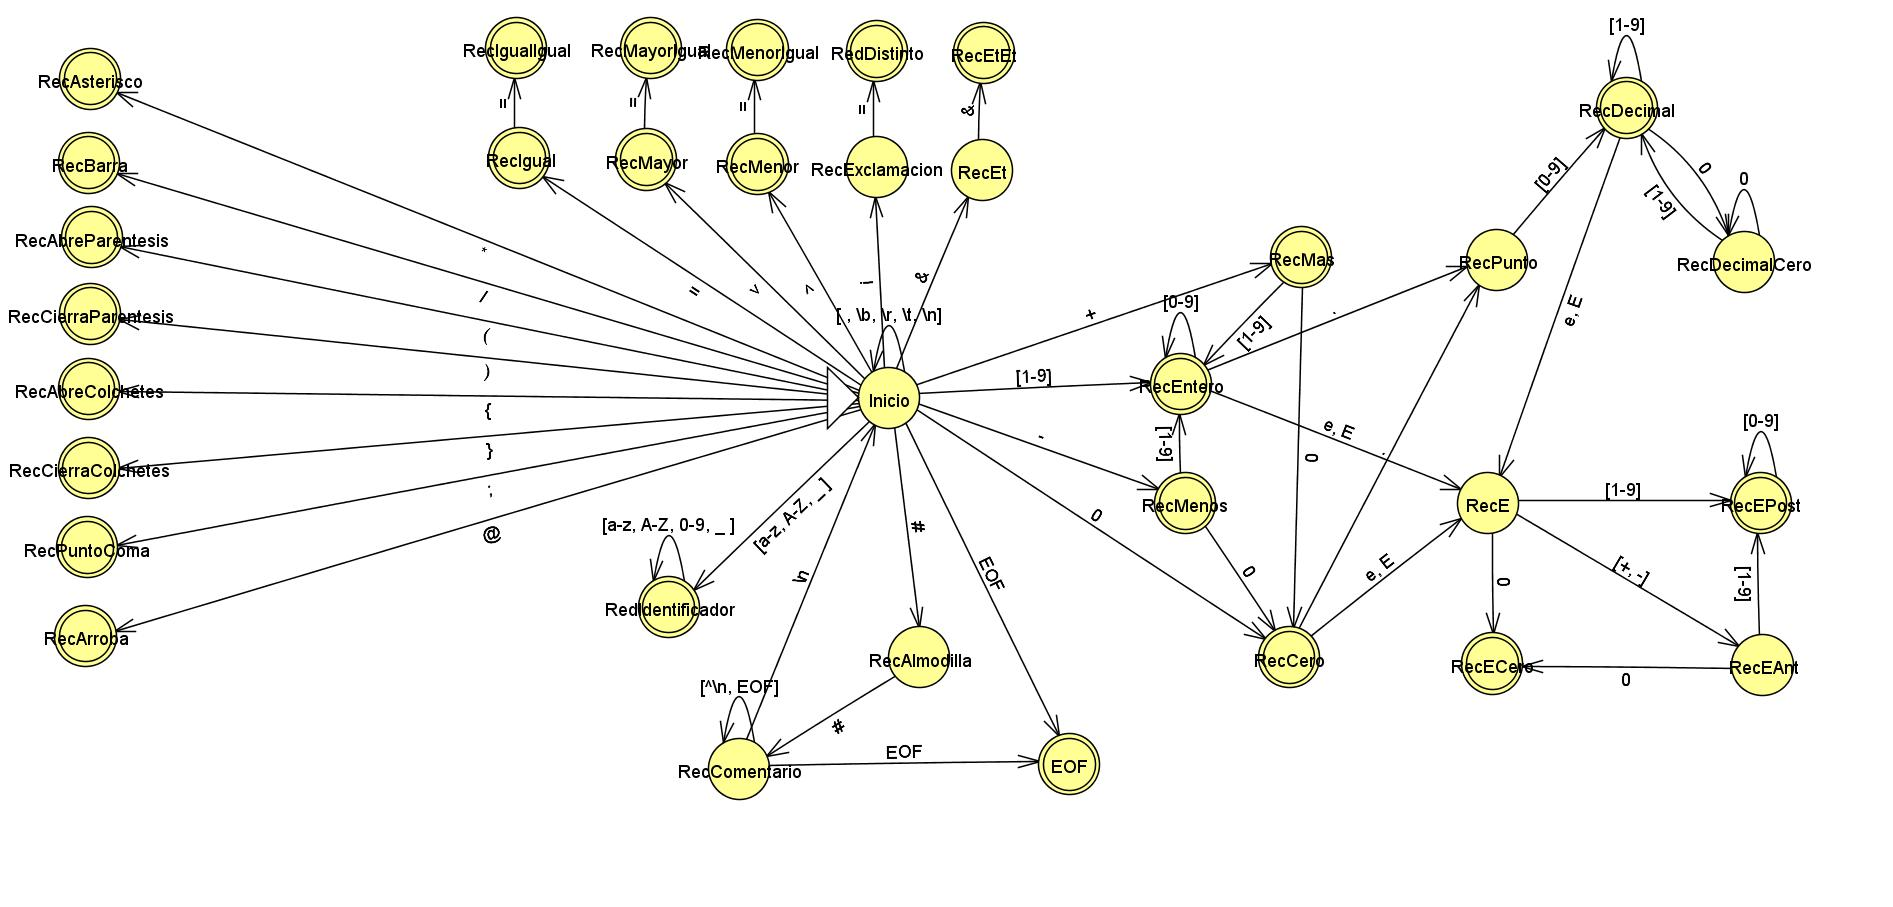
\includegraphics[width=0.7\linewidth]{Secciones/Hito1/Tiny0/Tiny0.jpg}
    \caption{AFD del analizador léxico de Tiny (0)}\label{fig:diag}
\end{figure}

\chapterA{Tiny}

\section{Introducción}
Para realizar este apartado nos hemos fijado en todas las funcionalidades que aparecen en el ``Apendice A''
del archivo ``fase1.pdf''. En los siguientes apartados definimos todas las clases que hay, su correspondiente especificación 
y un diagrama de transiciones.

\section{Clases léxicas}

\subsection{Palabras reservadas}

\t Para poder analizar de manera correcta, será necesario establecer una clase léxica por cada palabra reservada. En el lenguaje de
esta práctica, \textit{Tiny (0)}, contamos con 6 palabras reservadas, 3 de ellas utilizadas para definir el tipo de las variables.
Tendremos pues, una palabra para las variables de tipo booleano, otra para las de tipo entero y una última para las reales. Además
de éstas tendremos 3 palabras utilizadas para las operaciones lógicas. Las palabras son las definidas a continuación, contando cada con
una clase léxica.

\begin{itemize}
    \item \textit{bool} $\rightarrow$ Variables booleanas.
    \item \textit{int} $\rightarrow$ Variables enteras.
    \item \textit{real} $\rightarrow$ Variables reales.
    \item \textit{and} $\rightarrow$ Conjunción lógica.
    \item \textit{or} $\rightarrow$ Disyunción lógica.
    \item \textit{not} $\rightarrow$ Negación lógica.
    \item \textit{true} $\rightarrow$ Valor booleano cierto.
    \item \textit{false} $\rightarrow$ Valor booleano falso.
\end{itemize}

\subsection{Literales}

\begin{itemize}
    \item \textbf{Literales enteros.} Opcionalmente empiezan con un signo más (+) o menos (-), y después debe aparecer una
        secuencia (que empieza por un número distinto de 0) de 1 o más dígitos. Su clase léxica será \textit{literalEntero}.
    \item \textbf{Literales reales.}Empieza con una parte entera seguida de una parte decimal, exponecial o parte decimal seguida de exponecial. La parte decimal comienza con el signo punto (.) seguido de una secuencia (que puede ser sólo un 0 o números que no acaben en 0) de 1 o más dígitos. Por último, y también opcionalmente, puede aparecer una parte exponencial que se indica con (e) o (E), seguida de una parte entera con o sin parte decimal. Su clase léxica será \textit{literalReal}.
\end{itemize}

\subsection{Identificadores}

Los identificadores nos sirven para poder ponerle un nombre a las variables. Éstos deben comenzar por un subrayado (\_) o una letra, seguida de una secuencia de 0 o más
subrayados, dígitos o letras. Su clase léxica será \textit{identificador}.

\subsection{Símbolos de operación y puntuación}

Cada uno de ellos tendrá su propia clase léxica. En el subconjunto del lenguaje en el que trabajamos, \textit{Tiny (0)}, contamos con
las siguientes clases:

\begin{itemize}
    \item \textbf{Suma.} Se representa con el símbolo más (+). Su clase léxica será \textit{operadorSuma}.
    \item \textbf{Resta.} Se representa con el símbolo símbolo menos (-). Su clase léxica será \textit{operadorResta}.
    \item \textbf{Multiplicación.} Se representa con el símbolo asterisco (*). Su clase léxica será \textit{operadorMul}.
    \item \textbf{División.} Se representa con el símbolo barra (/). Su clase léxica será \textit{operadorDiv}.
    \item \textbf{Menor.} Se representa con el símbolo menor que (<). Su clase léxica será \textit{operadorMenor}.
    \item \textbf{Mayor.} Se representa con el símbolo mayor que (>). Su clase léxica será \textit{operadorMayor}.
    \item \textbf{Igual.} Se representa con dos símbolos de igualdad seguidos (==). Su clase léxica será \textit{operadorIgual}.
    \item \textbf{Menor o igual.} Se representa con el símbolo menor que seguido del símbolo de igualdad (<=). Su clase léxica será \textit{operadorMenIgual}.
    \item \textbf{Mayor o igual.} Se representa con el símbolo mayor que seguido del símbolo de igualdad (>=). Su clase léxica será \textit{operadorMayIgual}.
    \item \textbf{Asignación.} Se representa con un símbolo de igualdad (=). Su clase léxica será \textit{operadorAsig}.
    \item \textbf{Final.} Se representa con el símbolo ampersand dos veces consecutivas (\&\&). Su clase léxica será \textit{final}.
    \item \textbf{Paréntesis de apertura.} Se representa con el símbolo del paréntesis de apertura (``('', sin comillas). Su clase léxica será \textit{parentesisAp}.
    \item \textbf{Paréntesis de cierre.} Se representa con el símbolo del paréntesis de cierre (``)'', sin comillas). Su clase léxica será \textit{parentesisCi}.
    \item \textbf{Llave de apertura.} Se representa con el símbolo de la llave de apertura (``\{'', sin comillas). Su clase léxica será \textit{LlaveAp}.
    \item \textbf{Llave de cierre.} Se representa con el símbolo de la llave de cierre (``\}'', sin comillas). Su clase léxica será \textit{LlaveCi}.
    \item \textbf{Punto y coma.} Se representa con el símbolo punto y coma (;). Su clase léxica será \textit{puntoYComa}.
    \item \textbf{Coma.} Se representa con el símbolo coma (,). Su clase léxica será \textit{coma}.
\end{itemize}


\section{Especificación formal del léxico}


\subsection{Definiciones auxiliares.}
    
\begin{math}
    letra \longrightarrow [\textbf a -\textbf z,\textbf A - \textbf Z]\\
    digitoPositivo \longrightarrow [\textbf 1 - \textbf 9]\\
    digito \longrightarrow {digitoPositivo}|0\\
    parteEntera \longrightarrow [\backslash{+},\backslash{-}]?(\{digitoPositivo\} \; \{digito\}*|0)\\
    parteDecimal \longrightarrow (\{digito\}* \; \{digitoPositivo\}|0)\\
    parteExponencial \longrightarrow (e|E) parteEntera\\
\end{math}

\subsection{Definiciones de cadenas ignorables.}

\begin{math}
    separador \longrightarrow [\;\backslash{t}\backslash{r}\backslash{b}\backslash{n}]\\
    comentario \longrightarrow \#\#[\;\hat{}\;(\backslash{n}|\textbf{EOF})]*\\
\end{math}

\subsection{Definiciones léxicas.}

\begin{math}
    bool \longrightarrow (b|B)(o|O)(o|O)(l|L)\\
    int \longrightarrow (i|I)(n|N)(t|T)\\
    real \longrightarrow (r|R)(e|E)(a|A)(l|L)\\
    string \longrightarrow (s|S)(t|T)(r|R)(i|I)(n|N)(g|G)\\
    and \longrightarrow (a|A)(n|N)(d|D)\\
    or \longrightarrow (o|O)(r|R)\\
    not \longrightarrow (n|N)(o|O)(t|T)\\
    true \longrightarrow (t|T)(r|R)(u|U)(e|E)\\
    false \longrightarrow (f|F)(a|A)(l|L)(s|S)(e|E)\\
    null \longrightarrow (n|N)(u|U)(l|L)(l|L)\\
    proc \longrightarrow (p|P)(r|R)(o|O)(c|C)\\
    if \longrightarrow (i|I)(f|F)\\
    else \longrightarrow (e|E)(l|L)(s|S)(e|E)\\
    while \longrightarrow (w|W)(h|H)(i|I)(l|L)(e|E)\\
    struct \longrightarrow (s|S)(t|T)(r|R)(u|U)(c|C)(t|T)\\
    new \longrightarrow (n|N)(e|E)(w|W)\\
    delete \longrightarrow (d|D)(e|E)(l|L)(e|E)(t|T)(e|E)\\
    read \longrightarrow (r|R)(e|E)(a|A)(d|D)\\
    write \longrightarrow (w|W)(r|R)(i|I)(t|T)(e|E)\\
    nl \longrightarrow (n|N)(l|L)\\
    type \longrightarrow (t|T)(y|Y)(p|P)(e|E)\\
    call \longrightarrow (c|C)(a|A)(l|L)(l|L)\\
    literalEntero \longrightarrow \{parteEntera\}\\
    literalReal \longrightarrow \{parteEntera\}(\backslash{.}\{parteDecimal\}|\{parteExponencial\}|\backslash{.}\{parteDecimal\}\;\{parteExponencial\})\\
    identificador \longrightarrow (\_|letra)(letra|digito|\_)*\\
    literalCadena\longrightarrow ``[\;\hat{}\;''\;]*''\\
    suma \longrightarrow \backslash{+}\\
    resta \longrightarrow \; -\\
    mul \longrightarrow \; \backslash{*}\\
    div \longrightarrow \; /\\
    modulo \longrightarrow \%\\
    menor \longrightarrow \; <\\
    mayor \longrightarrow \; >\\
    igual \longrightarrow \; ==\\
    menorIgual \longrightarrow \; <=\\
    mayorIgual \longrightarrow \; >=\\
    asig \longrightarrow \; =\\
    finalAsig \longrightarrow \&\&\\
    parenApert \longrightarrow \; (\\
    parenCierre \longrightarrow \; )\\
    llaveApert \longrightarrow \; \backslash{\{}\\
    llaveCierre \longrightarrow \; \backslash{\}}\\
    puntoComa \longrightarrow \; ;\\
    coma \longrightarrow \; ,\\
    punto \longrightarrow \; .\\
    arroba \longrightarrow \; @\\
    indireccion \longrightarrow \; \backslash{\hat{}}\\
    final \longrightarrow \&\&\\
    paramRef \longrightarrow \&\\
    llaveApert \longrightarrow \; \{\\
    llaveCierre \longrightarrow \; \}\\
    corcheteApert \longrightarrow \; [\\
    corcheteCierre \longrightarrow \; ]\\
\end{math}




\chapterA{Tiny (0)}

\section{Funciones para el conjunto de pares de tipos}

\begin{itemize}
    \item \texttt{nuevoConjunto()}: Crea un conjunto vacío para almacenar los pares de tipos
    \item \texttt{contiene(set,tipo0,tipo1)}: Comprueba si el conjunto \texttt{set} contiene ya una entrada para el par (\texttt{tipo0}, \texttt{tipo1}).
    \item \texttt{inserta(set,tipo0,tipo1)}: Inserta el par (\texttt{tipo0}, \texttt{tipo1}) en el conjunto \texttt{set}.
\end{itemize}

\section{Funciones de procesamiento}

var set

\begin{math}
    \textbf{tipado}(\textbf{bloque}(SecDecs, \; SecIs)): \\
        \phantom{---} \textbf{tipado}(SecDecs) \\
        \phantom{---} \textbf{tipado}(SecIs) \\
        \phantom{---} \$.tipo \; = \; \textbf{ambos\_ok}(SecDecs.tipo, \; SecIs.tipo)
\end{math}

\subsection{Declaraciones}

\begin{math}
    \textbf{tipado}(\textbf{si\_decs}(LDecs)): \\
        \phantom{---} \textbf{tipado}(LDecs) \\
        \phantom{---} \$.tipo \; = \; LDecs.tipo \\
    \\
    \textbf{tipado}(\textbf{no\_decs()}): \\
        \phantom{---} \$.tipo \; = \; ok \\
    \\
    \textbf{tipado}(\textbf{muchas\_decs}(LDecs, \; Dec)): \\
        \phantom{---} \textbf{tipado}(LDecs) \\
        \phantom{---} \textbf{tipado}(Dec) \\
        \phantom{---} \$.tipo \; = \; \textbf{ambos\_ok}(LDecs.tipo, \; Dec.tipo) \\
    \\
    \textbf{tipado}(\textbf{una\_dec}(Dec)): \\
        \phantom{---} \textbf{tipado}(Dec) \\
        \phantom{---} \$.tipo \; = \; Dec.tipo \\
    \\
    \textbf{tipado}(\textbf{dec\_base}(TipoNom)): \\
        \phantom{---} \$.tipo \; = \; ok \\
    \\
    \textbf{tipado}(\textbf{dec\_type}(TipoNom)): \\
        \phantom{---} \$.tipo \; = \; ok \\
    \\
    \textbf{tipado}(\textbf{dec\_proc}(iden, \; ParamFs, \; Bloq)): \\
        \phantom{---} \textbf{tipado}(Bloq) \\
        \phantom{---} \$.tipo \; = \; Bloq.tipo
\end{math}

\subsection{Instrucciones}

\begin{math}
    \textbf{tipado}(\textbf{si\_ins}(LIs)): \\
        \phantom{---} \textbf{tipado}(LIs) \\
        \phantom{---} \$.tipo \; = \; LIs.tipo \\
    \\
    \textbf{tipado}(\textbf{no\_ins()}): \\
        \phantom{---} \$.tipo \; = \; ok \\
    \\
    \textbf{tipado}(\textbf{muchas\_ins}(LIs, \; I)): \\
        \phantom{---} \textbf{tipado}(LIs) \\
        \phantom{---} \textbf{tipado}(I) \\
        \phantom{---} \$.tipo \; = \; \textbf{ambos\_ok}(LIs.tipo, \; I.tipo) \\
    \\
    \textbf{tipado}(\textbf{una\_ins}(I)): \\
        \phantom{---} \textbf{tipado}(I) \\
        \phantom{---} \$.tipo \; = \; I.tipo \\
    \\
    \textbf{tipado}(\textbf{ins\_eval}(Exp)): \\
        \phantom{---} \textbf{tipado}(Exp) \\
        \phantom{---} if \; Exp.tipo \; != \; error \; then \\
            \phantom{------} \$.tipo \; = \; ok \\
        \phantom{---} else \\
            \phantom{------} \$.tipo \; = \; error \\
        \phantom{---} endif \\
    \\
    \textbf{tipado}(\textbf{ins\_if}(Exp, \; Bloq)): \\
        \phantom{---} \textbf{tipado}(Exp) \\
        \phantom{---} \textbf{tipado}(Bloq) \\
        \phantom{---} if \; \textbf{ref!}(Exp.tipo) \; == \; tipo\_bool() \; \land \; Bloq.tipo \; == \; ok \; then \\
            \phantom{------} \$.tipo \; = \; ok \\
        \phantom{---} else \\
            \phantom{------} \$.tipo \; = \; error \\
            \phantom{------} \textbf{error} \\
        \phantom{---} endif \\
    \\
    \textbf{tipado}(\textbf{ins\_if\_else}(I, \; Bloq)): \\
        \phantom{---} \textbf{tipado}(I) \\
        \phantom{---} \textbf{tipado}(Bloq) \\
        \phantom{---} \$.tipo \; = \; \textbf{ambos\_ok}(I.tipo, \; Bloq.tipo) \\
    \\
    \textbf{tipado}(\textbf{ins\_while}(Exp, \; Bloq)): \\
        \phantom{---} \textbf{tipado}(Exp) \\
        \phantom{---} \textbf{tipado}(Bloq) \\
        \phantom{---} if \; \textbf{ref!}(Exp.tipo) \; == \; tipo\_bool() \; \land \; Bloq.tipo \; == \; ok \; then \\
            \phantom{------} \$.tipo \; = \; ok \\
        \phantom{---} else \\
            \phantom{------} \$.tipo \; = \; error \\
            \phantom{------} \textbf{error} \\
        \phantom{---} endif \\
    \\
    \textbf{tipado}(\textbf{ins\_read}(Exp)): \\
        \phantom{---} \textbf{tipado}(Exp) \\
        \phantom{---} let \; T \; = \; \textbf{ref!}(Exp.tipo) \; in \\
        \phantom{------} if \; T \; == \; tipo\_int() \; \lor \\
        \phantom{--------} T \; == \; tipo\_real() \; \lor \\
        \phantom{--------} T \; == \; tipo\_string() \; then \\
            \phantom{---------} if \; \textbf{es\_designador}(Exp) \; then \\
                \phantom{------------} \$.tipo \; = \; ok \\
            \phantom{---------} else \\
                \phantom{------------} \$.tipo \; = \; error \\
                \phantom{------------} \textbf{error} \\
            \phantom{---------} endif \\
        \phantom{------} else \\
            \phantom{---------} \$.tipo \; = \; error \\
            \phantom{---------} \textbf{error} \\
        \phantom{------} endif \\
        \phantom{---} end \; let \\
    \\
    \textbf{tipado}(\textbf{ins\_write}(Exp)): \\
        \phantom{---} \textbf{tipado}(Exp) \\
        \phantom{---} let \; T \; = \; \textbf{ref!}(Exp.tipo) \; in \\
        \phantom{------} if \; (T \; == \; tipo\_int() \; \lor \\
        \phantom{--------} T \; == \; tipo\_real() \; \lor \\
        \phantom{--------} T \; == \; tipo\_bool() \; \lor \\
        \phantom{--------}  T \; == \; tipo\_string()) \; then \\
            \phantom{---------} \$.tipo \; = \; ok \\
        \phantom{------} else \\
            \phantom{---------} \$.tipo \; = \; error \\
            \phantom{---------} \textbf{error} \\
        \phantom{------} endif \\
        \phantom{---} end \; let \\
    \\
    \textbf{tipado}(\textbf{ins\_nl}()): \\
        \phantom{---} \$.tipo \; = \; ok \\
    \\
    \textbf{tipado}(\textbf{ins\_new}(Exp)): \\
        \phantom{---} \textbf{tipado}(Exp) \\
        \phantom{---} if \; \textbf{ref!}(Exp.tipo) \; == \; tipo\_indir(\_) \; then \\
            \phantom{------} \$.tipo \; = \; ok \\
        \phantom{---} else \\
            \phantom{------} \$.tipo \; = \; error \\
            \phantom{------} \textbf{error} \\
        \phantom{---} endif \\
    \\
    \textbf{tipado}(\textbf{ins\_delete}(Exp)): \\
        \phantom{---} \textbf{tipado}(Exp) \\
        \phantom{---} if \; \textbf{ref!}(Exp.tipo) \; == \; tipo\_indir(\_) \; then \\
            \phantom{------} \$.tipo \; = \; ok \\
        \phantom{---} else \\
            \phantom{------} \$.tipo \; = \; error \\
            \phantom{------} \textbf{error} \\
        \phantom{---} endif \\
    \\
    \textbf{tipado}(\textbf{ins\_call}(iden, \; ParamRs)): \\
        \phantom{---} \textbf{tipado}(ParamRs) \\
        \phantom{---} if \; \$.vinculo \; != \; dec\_proc(\_, \; ParamFs, \; \_) \; then \\
            \phantom{------} if \; ParamRs \; == \; no\_params\_r() \; \land \; ParamFs \; == \; no\_params\_f() \; then \\
                \phantom{---------} \$.tipo = ok \\
            \phantom{------} else \; if \; ParamRs \; == \; si\_params\_r(LParamRs) \; \land \; ParamFs \; == \; si\_params\_f(LParamsFs) \; then \\
                \phantom{---------} if \; \textbf{num\_params}(LParamRs, \; LParamFs) \; then \\
                    \phantom{------------} if \; \textbf{compatibles\_params}(LParamRs, \; LParamFs) \; then \\
                        \phantom{---------------} \$.tipo = ok \\
                    \phantom{------------} else \\
                        \phantom{---------------} \$.tipo \; = \; error \\
                    \phantom{------------} endif \\
                \phantom{---------} else \\
                    \phantom{------------} \$.tipo \; = \; error \\
                    \phantom{------------} \textbf{error} \\
                \phantom{---------} endif \\
            \phantom{------} else \\
                \phantom{---------} \$.tipo \; = \; error \\
                \phantom{---------} \textbf{error} \\
            \phantom{------} endif \\
        \phantom{---} else \\
            \phantom{------} \$.tipo \; = \; error \\
            \phantom{------} \textbf{error} \\
        \phantom{---} endif \\
    \\
    \textbf{tipado}(\textbf{ins\_bloque}(Bloq)): \\
        \phantom{---} \textbf{tipado}(Bloq) \\
        \phantom{---} \$.tipo \; = \; Bloq.tipo \\
    \\
    \textbf{tipado}(\textbf{si\_params\_r}(LParamRs)): \\
        \phantom{---} \textbf{tipado}(LParamRs) \\
    \\
    \textbf{tipado}(\textbf{no\_params\_r()}): \textbf{noop} \\
    \\
    \textbf{tipado}(\textbf{muchos\_params\_r}(LParamRs, \; Exp)): \\
        \phantom{---} \textbf{tipado}(LParamRs) \\
        \phantom{---} \textbf{tipado}(Exp) \\
    \\
    \textbf{tipado}(\textbf{un\_param\_r}(Exp)): \\
        \phantom{---} \textbf{tipado}(Exp)
\end{math}

\subsection{Expresiones}

\begin{math}
    \textbf{tipado}(\textbf{exp\_asig}(Opnd0, \; Opnd1)): \\
        \phantom{---} \textbf{tipado}(Opnd0) \\
        \phantom{---} \textbf{tipado}(Opnd1) \\
        \phantom{---} if \; \textbf{es\_designador}(Opnd0) \; then \\
            \phantom{------} if \; \textbf{compatibles}(Opnd0.tipo, \; Opnd1.tipo) \; then \\
                \phantom{---------} \$.tipo \; = \; ok \\
            \phantom{------} else \\
                \phantom{---------} \$.tipo \; = \; error \\
                \phantom{---------} \textbf{error} \\
            \phantom{------} endif \\
        \phantom{---} else \\
            \phantom{------} \$.tipo \; = \; error \\
            \phantom{------} \textbf{error} \\
        \phantom{---} endif \\
    \\
    \textbf{tipado}(\textbf{exp\_menor}(Opnd0, \; Opnd1)): \\
        \phantom{---} \textbf{tipado\_rel}(Opnd0, \; Opnd1, \; \$) \\
    \\
    \textbf{tipado}(\textbf{exp\_menor\_ig}(Opnd0, \; Opnd1)): \\
        \phantom{---} \textbf{tipado\_rel}(Opnd0, \; Opnd1, \; \$) \\
    \\
    \textbf{tipado}(\textbf{exp\_mayor}(Opnd0, \; Opnd1)): \\
        \phantom{---} \textbf{tipado\_rel}(Opnd0, \; Opnd1, \; \$) \\
    \\
    \textbf{tipado}(\textbf{exp\_mayor\_ig}(Opnd0, \; Opnd1)): \\
        \phantom{---} \textbf{tipado\_rel}(Opnd0, \; Opnd1, \; \$) \\
    \\
    \textbf{tipado}(\textbf{exp\_ig}(Opnd0, \; Opnd1)): \\
        \phantom{---} \textbf{tipado\_rel}(Opnd0, \; Opnd1, \; \$) \\
    \\
    \textbf{tipado}(\textbf{exp\_dist}(Opnd0, \; Opnd1)): \\
        \phantom{---} \textbf{tipado\_rel}(Opnd0, \; Opnd1, \; \$) \\
    \\
    \textbf{tipado}(\textbf{exp\_suma}(Opnd0, \; Opnd1)): \\
        \phantom{---} \textbf{tipado\_arit}(Opnd0, \; Opnd1, \; \$) \\
    \\
    \textbf{tipado}(\textbf{exp\_resta}(Opnd0, \; Opnd1)): \\
        \phantom{---} \textbf{tipado\_arit}(Opnd0, \; Opnd1, \; \$) \\
    \\
    \textbf{tipado}(\textbf{exp\_and}(Opnd0, \; Opnd1)): \\
    \phantom{---} \textbf{tipado\_logic}(Opnd0, \; Opnd1, \; \$) \\
    \\
    \textbf{tipado}(\textbf{exp\_or}(Opnd0, \; Opnd1)): \\
        \phantom{---} \textbf{tipado\_logic}(Opnd0, \; Opnd1, \; \$) \\
    \\
    \textbf{tipado}(\textbf{exp\_mul}(Opnd0, \; Opnd1)): \\
        \phantom{---} \textbf{tipado\_arit}(Opnd0, \; Opnd1, \; \$) \\
    \\
    \textbf{tipado}(\textbf{exp\_div}(Opnd0, \; Opnd1)): \\
        \phantom{---} \textbf{tipado\_arit}(Opnd0, \; Opnd1, \; \$) \\  
    \\
    \textbf{tipado}(\textbf{exp\_mod}(Opnd0, \; Opnd1)): \\
        \phantom{---} \textbf{tipado}(Opnd0) \\
        \phantom{---} \textbf{tipado}(Opnd1) \\
        \phantom{---} if \; \textbf{ref!}(Opnd0.tipo) \; == \; tipo\_int() \; \land \\
        \phantom{-----} \textbf{ref!}(Opnd1.tipo) \; == \; tipo\_int() \; then \\
            \phantom{------} \$.tipo \; = \; tipo\_int() \\
        \phantom{---} else \\
            \phantom{------} \$.tipo \; = \; error \\
            \phantom{------} \textbf{aviso\_error\_bin}(T0, \; T1) \\
        \phantom{---} endif \\
    \\
    \textbf{tipado}(\textbf{exp\_menos}(Opnd)): \\
        \phantom{---} \textbf{tipado}(Opnd) \\
        \phantom{---} let \; T \; = \; \textbf{ref!}(Opnd.tipo) \; in \\
        \phantom{------} if \; T \; == \; tipo\_int() \; then \\
            \phantom{---------} \$.tipo \; = \; tipo\_int() \\
        \phantom{------} else \; if \; T \; == \; tipo\_real() \; then \\
            \phantom{---------} \$.tipo \; = \; tipo\_real() \\
        \phantom{------} else \\
            \phantom{---------} \$.tipo \; = \; error \\
            \phantom{---------} \textbf{aviso\_error\_un}(T) \\
        \phantom{------} endif \\
        \phantom{---} end \; let \\
    \\
    \textbf{tipado}(\textbf{exp\_not}(Opnd)): \\
        \phantom{---} \textbf{tipado}(Opnd) \\
        \phantom{---} if \; \textbf{ref!}(Opnd.tipo) \; == \; tipo\_bool() \; then \\
            \phantom{------} \$.tipo \; = \; tipo\_bool() \\
        \phantom{---} else \\
            \phantom{------} \$.tipo \; = \; error \\
            \phantom{------} \textbf{aviso\_error\_un}(T) \\
        \phantom{---} endif \\
    \\
    \textbf{tipado}(\textbf{exp\_index}(Opnd0, \; Opnd1)): \\
        \phantom{---} \textbf{tipado}(Opnd0) \\
        \phantom{---} \textbf{tipado}(Opnd1) \\
        \phantom{---} if \; \textbf{ref!}(Opnd0.tipo) \; == \; tipo\_array(Tipo, \; \_) \; \land \\
        \phantom{-----} \textbf{ref!}(Opnd1.tipo) \; == \; tipo\_int() \; then \\
            \phantom{------} \$.tipo \; = \; tipo\_array(Tipo, \; \_) \\
        \phantom{---} else \\
            \phantom{------} \$.tipo \; = \; error \\
            \phantom{------} \textbf{error} \\
        \phantom{---} endif \\
    \\
    \textbf{tipado}(\textbf{exp\_reg}(Opnd, iden)): \\
        \phantom{---} \textbf{tipado}(Opnd) \\
        \phantom{---} if \; \textbf{ref!}(Opnd.tipo) \; == \; tipo\_struct(LCampos) \; then \\
            \phantom{------} let \; C \; = \; \textbf{campo\_struct}(LCampos, \; iden) \; in \\
                \phantom{---------} if \; C \; == \; error \; then \\
                    \phantom{------------} \textbf{error} \\
                \phantom{---------} endif \\
                \phantom{---------} \$.tipo \; = \; C \\
            \phantom{------} end \; let \\
        \phantom{---} else \\
            \phantom{------} \$.tipo \; = \; error \\
            \phantom{------} \textbf{error} \\
        \phantom{---} endif \\
    \\
    \textbf{tipado}(\textbf{exp\_indir}(Opnd)): \\
        \phantom{---} \textbf{tipado}(Opnd) \\
        \phantom{---} if \; \textbf{ref!}(Opnd.tipo) \; == \; tipo\_indir(Tipo) \; then \\
            \phantom{------} \$.tipo \; = \; tipo\_indir(Tipo) \\
        \phantom{---} else \\
            \phantom{------} \$.tipo \; = \; error \\
            \phantom{------} \textbf{error} \\
        \phantom{---} endif \\
    \\
    \textbf{tipado}(\textbf{exp\_entero}(litEntero)): \\
        \phantom{---} \$.tipo \; = \; tipo\_int() \\
    \\
    \textbf{tipado}(\textbf{exp\_real}(litReal)): \\
        \phantom{---} \$.tipo \; = \; tipo\_real() \\
    \\
    \textbf{tipado}(\textbf{exp\_true}()): \\
        \phantom{---} \$.tipo \; = \; tipo\_bool() \\
    \\
    \textbf{tipado}(\textbf{exp\_false}()): \\
        \phantom{---} \$.tipo \; = \; tipo\_bool() \\
    \\
    \textbf{tipado}(\textbf{exp\_cadena}(litCadena)): \\
        \phantom{---} \$.tipo \; = \; tipo\_string() \\
    \\
    \textbf{tipado}(\textbf{exp\_iden}(iden)): \\
        \phantom{---} if \; \$.vinculo \; = dec\_base(TipoNom) \; then \\
            \phantom{------} let \; TipoNom \; = \; TipoNom(Tipo, \; iden) in \\
                \phantom{---------} \$.tipo \; = \; Tipo \\
            \phantom{------} end \; let \\
        \phantom{---} else \; if \; \$.vinculo \; = si\_refparam\_f(Tipo,\; \_) \; \lor \; \$.vinculo \; = no\_refparam\_f(Tipo,\; \_) \; then \\
            \phantom{------} \$.tipo \; = \; Tipo \\
        \phantom{---} else \\
            \phantom{------} \$.tipo \; = \; error \\
            \phantom{------} \textbf{error} \\
        \phantom{---} endif \\
    \\
    \textbf{tipado}(\textbf{exp\_null}()): \\
        \phantom{---} \$.tipo \; = \; null \\
    \\
    \textbf{tipado\_arit}(Opnd0, \; Opnd1, \; Exp): \\
        \phantom{---} \textbf{tipado}(Opnd0) \\
        \phantom{---} \textbf{tipado}(Opnd1) \\
        \phantom{---} let \; T0 \; = \; \textbf{ref!}(Opnd0.tipo) \; \land \; T1 \; = \; \textbf{ref!}(Opnd1.tipo) \; in \\
        \phantom{------} if \; T0 \; == \; tipo\_int() \; \land \\
        \phantom{--------} T1 \; == \; tipo\_int() \; then \\
            \phantom{---------} Exp.tipo \; = \; tipo\_int() \\
        \phantom{------} else \; if \; (T0 \; == \; tipo\_real() \; \lor \\
        \phantom{---------} T0 \; == \; tipo\_int()) \; \land \\
        \phantom{---------} (T1 \; == \; tipo\_real() \lor \\
        \phantom{---------} T1 \; == \; tipo\_int()) \; then \\
            \phantom{---------} Exp.tipo \; = \; tipo\_real() \\
        \phantom{------} else \\
            \phantom{---------} Exp.tipo \; = \; error \\
            \phantom{---------} \textbf{aviso\_error\_bin}(T0, \; T1) \\
        \phantom{------} endif \\
        \phantom{---} end \; let \\
    \\
    \textbf{tipado\_logic}(Opnd0, \; Opnd1, \; Exp): \\
        \phantom{---} \textbf{tipado}(Opnd0) \\
        \phantom{---} \textbf{tipado}(Opnd1) \\
        \phantom{---} let \; T0 \; = \; \textbf{ref!}(Opnd0.tipo) \; \land \; T1 \; = \; \textbf{ref!}(Opnd1.tipo) \; in \\
        \phantom{------} if \; T0 \; == \; tipo\_bool() \; \land \\
        \phantom{--------} T1 \; == \; tipo\_bool() \; then \\
            \phantom{---------} Exp.tipo \; = \; tipo\_bool() \\
        \phantom{------} else \\
            \phantom{---------} Exp.tipo \; = \; error \\
            \phantom{---------} \textbf{aviso\_error\_bin}(T0, \; T1) \\
        \phantom{------} endif \\
        \phantom{---} end \; let \\
    \\
    \textbf{tipado\_rel}(Opnd0, \; Opnd1, \; Exp): \\
        \phantom{---} \textbf{tipado}(Opnd0) \\
        \phantom{---} \textbf{tipado}(Opnd1) \\
        \phantom{---} let \; T0 \; = \; \textbf{ref!}(Opnd0.tipo) \; \land \; T1 \; = \; \textbf{ref!}(Opnd1.tipo) \; in \\
        \phantom{------} if \; (T0 \; == \; tipo\_int() \; \lor \\
        \phantom{--------} T0 \; == \; tipo\_real()) \; \land \\
        \phantom{-------} (T1 \; == \; tipo\_int() \; \lor \\
        \phantom{--------} T1 \; == \; tipo\_real()) \; then \\
            \phantom{---------} Exp.tipo \; = \; tipo\_bool() \\
        \phantom{------} else \; if \; T0 \; == \; tipo\_bool() \; \land \\
        \phantom{--------} T1 \; == \; tipo\_bool() \; then \\
            \phantom{---------} Exp.tipo \; = \; tipo\_bool() \\
        \phantom{------} else \; if \; T0 \; == \; tipo\_string() \; \land \\
        \phantom{--------} T1 \; == \; tipo\_string() \; then \\
            \phantom{---------} Exp.tipo \; = \; tipo\_string() \\
        \phantom{------} else \\
            \phantom{--------} if \; Exp \; == \; exp\_ig(\_, \; \_) \; \lor \\
            \phantom{---------} Exp \; == \; exp\_dist(\_, \; \_) \; then \\
            \phantom{-----------} \textbf{tipado\_rel\_indir}(Opnd0, \; Opnd1, \; Exp) \\
            \phantom{--------} else \\
            \phantom{-----------} Exp.tipo \; = \; error \\
            \phantom{-----------} \textbf{aviso\_error\_bin}(T0, \; T1) \\
            \phantom{--------} endif \\
        \phantom{------} endif \\
        \phantom{---} end \; let \\
    \\
    \textbf{tipado\_rel\_indir}(T0, \; T1, \; Exp): \\
        \phantom{---} if \; (T0 \; == \; tipo\_indir() \; \lor \\
        \phantom{-----} T0 \; == \; null) \; \land \\
        \phantom{-----} (T1 \; == \; tipo\_indir() \; \land \\
        \phantom{-----} T1 \; == \; null) \; then \\
            \phantom{------} Exp.tipo \; = \; tipo\_bool() \\
        \phantom{----} else \\
            \phantom{------} Exp.tipo \; = \; error \\
            \phantom{------} \textbf{aviso\_error\_bin}(T0, \; T1) \\
        \phantom{---} endif
\end{math}

\section{Funciones auxiliares}

\begin{math}
    \textbf{aviso\_error\_bin}(T0, \; T1): \\
        \phantom{---} if \; T0 \; != \; error \; \land \; T1 \; != \; error \; then \\
            \phantom{------} \textbf{error} \\
        \phantom{---} endif \\
    \\
    \textbf{aviso\_error\_un}(T): \\
        \phantom{---} if \; T \; != \; error \; then \\
            \phantom{------} \textbf{error} \\
        \phantom{---} endif \\
    \\
    \textbf{ambos\_ok}(T0, \; T1): \\
        \phantom{---} if \; T0 \; == \; ok \; \land \; T1 \; == \; ok \; then \\
            \phantom{------} \textbf{return} \; ok \\
        \phantom{---} else \\
            \phantom{------} \textbf{return} \; error \\
        \phantom{---} endif \\
    \\
    \textbf{ref!}(T): \\
        \phantom{---} if \; T \; == \; tipo\_type(\_) \; then \\
            \phantom{------} let \; T.vinculo = dec\_type(Tipo, \; iden) \; in \\
                \phantom{---------} \textbf{return ref!}(Tipo) \\
            \phantom{------} end \; let \\
        \phantom{---} else \\
            \phantom{------} \textbf{return} \; T \\
        \phantom{---} endif \\
    \\
    \textbf{es\_designador}(E): \\
        \phantom{---} \textbf{return} \; E \; == \; exp\_iden(\_) \; \lor \\
        \phantom{-------} E \; == \; exp\_index(\_, \; \_) \; \lor \\
        \phantom{-------} E \; == \; exp\_reg(\_, \; \_) \; \lor \\
        \phantom{-------} E \; == \; exp\_indir(\_) \\
    \\
    \textbf{compatibles}(T0, \; T1): \\
        \phantom{---} set \; = \; \textbf{nuevoConjunto}() \\
        \phantom{---} \textbf{inserta}(set, \; T0, \; T1) \\
        \phantom{---} \textbf{return unificables}(T0, \; T1) \\
    \\
    \textbf{unificables}(T0, \; T1): \\
        \phantom{---} let \; T0' \; = \; \textbf{ref!}(T0) \; \land \; T1' \; = \; \textbf{ref!}(T1) \; in \\
        \phantom{------} if \; T0' \; == \; tipo\_array(Tipo_0, \; \_) \; \land \; T1' \; == \; tipo\_array(Tipo_1, \; \_) \; then \\
            \phantom{---------} \textbf{return son\_unificables}(Tipo_0, \; Tipo_1) \\
        \phantom{------} else \; if \; T0' \; == \; tipo\_struct(LCampos_0) \; \land \; T1' \; == \; tipo\_struct(LCampos_1) \; then \\
            \phantom{---------} \textbf{return son\_unificables\_struct}(LCampos_0, \; LCampos_1) \\
        \phantom{------} else \; if \; T0' \; == \; tipo\_indir(\_) \; \land \; T1' \; == \; null \; then \\
            \phantom{---------} \textbf{return} \; true \\
        \phantom{------} else \; if \; T0' \; == \; tipo\_indir(Tipo_0) \; \land \; T1' \; == \; tipo\_indir(Tipo_1) \; then \\
            \phantom{---------} \textbf{return son\_unificables}(Tipo_0, \; Tipo_1) \\
        \phantom{------} else \; if \; T0' \; == \; T1' \; \lor \; (T0' \; == \; tipo\_real() \; \land \; T1' \; == \; tipo\_int()) \; then \\
            \phantom{---------} \textbf{return} \; true \\
        \phantom{------} else \\
            \phantom{---------} \textbf{return} \; false \\
        \phantom{-----} endif \\
        \phantom{---} end \; let \\
    \\
    \textbf{son\_unificables\_struct}(LCampos0, \; LCampos1): \\
        \phantom{---} if \; LCampos0 \; == \; un\_campo(TipoNom_0) \; \land \; LCampos1 \; == \; un\_campo(TipoNom_1) \; then \\
            \phantom{------} let \; TipoNom_0 \; = \; TipoNom(Tipo_0, \; \_) \; \land \; TipoNom_1 \; = \; TipoNom(Tipo_1, \; \_) \\
            \phantom{---------} \textbf{return son\_unificables}(Tipo_0, \; Tipo_1) \\
            \phantom{------} end \; let \\
        \phantom{---} else \; if \; LCampos0 \; == \; muchos\_campos(LCampos_0, \; TipoNom_0) \; \land \\
        \phantom{-----}\; LCampos1 \; == \; muchos\_campos(LCampos_1, \;TipoNom_1) \; then \\
            \phantom{------} let \; TipoNom_0 \; = \; TipoNom(Tipo_0, \; \_) \; \land \; TipoNom_1 \; = \; TipoNom(Tipo_1, \; \_) \\
            \phantom{---------} \textbf{return son\_unificables}(Tipo_0, \; Tipo_1) \; \land \\
            \phantom{------------} \textbf{son\_unificables\_struct}(LCampos_0, \; LCampos_1) \\
            \phantom{------} end \; let \\
        \phantom{---} else \\
        \phantom{------} \textbf{return} \; false \\
        \phantom{---} endif \\
    \\
    \textbf{son\_unificables}(T0, \; T1): \\
        \phantom{---} if \; \textbf{contiene}(set, \; T0, \; T1) \; then \\
            \phantom{------} \textbf{return} \; true \\
        \phantom{---} else \\
            \phantom{------} \textbf{inserta}(set, \; T0, \; T1)\\
            \phantom{------} \textbf{return unificables}(T0, \; T1) \\
        \phantom{---} endif \\
    \\
    \textbf{campo\_struct}(LCampos, \; iden): \\
        \phantom{---} if \; LCampos \; == \; un\_campo(TipoNom_0) \; then \\
            \phantom{------} let \; TipoNom_0 \; = \; TipoNom(Tipo_0, \; iden_0) \\
                \phantom{--------} if \; iden \; == \; iden_0 \; then \\
                    \phantom{-----------} \textbf{return} \; Tipo_0 \\
                \phantom{--------} else \\
                    \phantom{-----------} \textbf{return} \; error \\
                \phantom{--------} endif \\
            \phantom{------} end \; let \\
        \phantom{---} else \; if \; LCampos \; == \; muchos\_campos(LCampos_0, \; TipoNom_0) \; then \\
            \phantom{------} let \; TipoNom_0 \; = \; TipoNom(Tipo_0, \; iden_0) \\
                \phantom{--------} if \; iden \; == \; iden_0 \; then \\
                    \phantom{-----------} \textbf{return} \; Tipo_0 \\
                \phantom{--------} else \\
                    \phantom{-----------} \textbf{return campo\_struct}(LCampos_0, iden) \\
                \phantom{--------} endif \\
            \phantom{------} end \; let \\
        \phantom{---} endif \\
    \\
    \textbf{num\_params}(LParamRs, \; LParamFs): \\
        \phantom{---} if \; LParamRs \; == \; un\_param\_r(\_) \; \land \; LParamFs \; == \; un\_param\_f(\_) \; then \\
            \phantom{------} \textbf{return} \; true \\
        \phantom{---} else \; if \; LParamRs \; == \; muchos\_params\_r(LParamRs_0, \; \_) \; \land \\
        \phantom{-----} LParamFs \; == \; muchos\_params\_f(LParamFs_0, \; \_) \; then \\
            \phantom{------} \textbf{return num\_params}(LParamRs_0 \; LParamFs_0) \\
        \phantom{---} else \\
            \phantom{------} \textbf{return} \; false \\
        \phantom{---} endif \\
    \\
    \textbf{compatibles\_params}(LParamRs, \; LParamFs): \\
        \phantom{---} if \; LParamRs \; == \; un\_param\_r(Exp) \; \land \; LParamFs \; == \; un\_param\_f(ParamF) \; then \\
            \phantom{------} \textbf{return param\_r\_f}(Exp, \; ParamF) \\
        \phantom{---} else \; if \; LParamRs \; == \; muchos\_params\_r(LParamRs_0, \; Exp) \; \land \\
        \phantom{-----} LParamFs \; == \; muchos\_params\_f(LParamFs_0, \; Tipo) \; then \\
            \phantom{------} \textbf{return param\_r\_f}(Exp, \; ParamF) \; \land \\
            \phantom{---------} \textbf{compatibles\_params}(LParamRs_0 \; LParamFs_0) \\
        \phantom{---} endif \\
    \\
    \textbf{param\_r\_f}(Exp, \; ParamF): \\
        \phantom{---} if \; ParamF \; == \; si\_refparam\_f(Tipo, \_) \; then \\
            \phantom{------} if \; \textbf{es\_designador}(Exp) \; then \\
                \phantom{---------} if \; ParamF \; == \; tipo\_real() \; then \\
                    \phantom{-----------} if \; Exp.tipo \; == \; tipo\_real() \; then \\
                        \phantom{---------------} \textbf{return} \; true \\
                    \phantom{-----------} else \\
                        \phantom{---------------} \textbf{error} \\
                        \phantom{---------------} \textbf{return} \; false \\
                    \phantom{-----------} endif \\
                \phantom{---------} else \\
                    \phantom{-----------} if \; \textbf{compatibles}(Tipo, \; Exp.tipo) \; then \\
                        \phantom{---------------} \textbf{return} \; true \\
                    \phantom{-----------} else \\
                        \phantom{---------------} \textbf{error} \\
                        \phantom{---------------} \textbf{return} \; false \\
                    \phantom{-----------} endif \\
                \phantom{---------} endif \\
            \phantom{------} else \\
                \phantom{---------} \textbf{error} \\
                \phantom{---------} \textbf{return} \; false \\
            \phantom{------} endif \\
        \phantom{---} else \\
            \phantom{-----} if \; \textbf{compatibles}(Tipo, \; Exp.tipo) \; then \\
                \phantom{---------} \textbf{return} \; true \\
            \phantom{-----} else \\
                \phantom{---------} \textbf{error} \\
                \phantom{---------} \textbf{return} \; false \\
            \phantom{-----} endif \\
        \phantom{---} endif
\end{math}


\section{Acondicionamiento}

Acondicionamos la gramática definida en la sección anterior. Ésto, con el fin de implementar un analizador
sintáctico descendente predictivo recursivo.

\begin{math}
    programa \longrightarrow \; bloque \\
    bloque \longrightarrow \; \{ seccion\_declaraciones\_opt \;\; seccion\_intrucciones\_opt \}
\end{math}

\subsection{Declaraciones}

\begin{math}
    seccion\_declaraciones\_opt \longrightarrow \; seccion\_declaraciones \; \&\& \\
    seccion\_declaraciones\_opt \longrightarrow \; \epsilon \\
    % RECURSION A IZQ 
    seccion\_declaraciones \longrightarrow \; declaracion \; resto\_sd \\
    resto\_sd \longrightarrow \; ; \; declaracion \; resto\_sd \\
    resto\_sd \longrightarrow \; \epsilon \\
    %
    declaracion \longrightarrow \; tipo\_nombre \\
    declaracion \longrightarrow \; \textbf{type} \; tipo\_nombre \\
    declaracion \longrightarrow \; \textbf{proc} \; \textbf{identificador} \; parametros\_formales \; bloque\\
    parametros\_formales \longrightarrow \; ( lista\_parametros\_opt ) \\
    lista\_parametros\_opt \longrightarrow \; lista\_parametros \\
    lista\_parametros\_opt \longrightarrow \; \epsilon \\ 
    % RECURSION A IZQ
    lista\_parametros \longrightarrow \; parametro \; resto\_lp \\
    resto\_lp \longrightarrow \; , \; parametro \; resto\_lp \\
    resto\_lp \longrightarrow \; \epsilon \\
    %
    parametro \longrightarrow \; tipo \; ref\_opt \; \textbf{identificador} \\
    ref\_opt \longrightarrow \; \& \\
    ref\_opt \longrightarrow \; \epsilon
\end{math}

\subsection{Tipos}

\begin{math}
    tipo\_nombre \longrightarrow \; tipo \; \textbf{identificador} \\
    tipo \longrightarrow \; tipo0 \\
    tipo0 \longrightarrow \; tipo0 \; tamano\_opt \\
    tipo0 \longrightarrow \; tipo1 \\
    tipo1 \longrightarrow \; \hat{} \; tipo1 \\
    tipo1 \longrightarrow \; tipo\_base \\
    tipo\_base \longrightarrow \; \textbf{struct} \; { lista\_campos } \\
    tipo\_base \longrightarrow \; \textbf{int} \\
    tipo\_base \longrightarrow \; \textbf{real} \\
    tipo\_base \longrightarrow \; \textbf{bool} \\
    tipo\_base \longrightarrow \; \textbf{string} \\
    tipo\_base \longrightarrow \; \textbf{identificador} \\
    tamano\_opt \longrightarrow \; [\textbf{literalEntero}] \\
    tamano\_opt \longrightarrow \; \epsilon \\
    % RECURSION A IZQ
    lista\_campos \longrightarrow \; tipo\_nombre \; resto\_lc \\
    resto\_lc \longrightarrow \; , \; tipo\_nombre \; resto\_lc \\
    resto\_lc \longrightarrow \; \epsilon
    %
\end{math}

\subsection{Instrucciones}

\begin{math}
    seccion\_intrucciones\_opt \longrightarrow \; seccion\_intrucciones \\
    seccion\_intrucciones\_opt \longrightarrow \; \epsilon \\
    seccion\_intrucciones \longrightarrow \; lista\_instrucciones \\
    % RECURSION A IZQ
    lista\_instrucciones \longrightarrow \; instruccion \; resto\_li \\
    resto\_li \longrightarrow \; ; \; instruccion \; resto\_li \\
    resto\_li \longrightarrow \; \epsilon \\
    %
    instruccion \longrightarrow \; @ \; expresion \\
    % FACTOR COMUN
    instruccion \longrightarrow \; if\_ins \; resto\_ii \\
    resto\_ii \longrightarrow \; else\_ins \\
    resto\_ii \longrightarrow \; \epsilon \\
    %
    instruccion \longrightarrow \; \textbf{while} \; exp\_bloque \\
    instruccion \longrightarrow \; \textbf{read} \; expresion \\
    instruccion \longrightarrow \; \textbf{write} \; expresion \\
    instruccion \longrightarrow \; \textbf{nl} \\
    instruccion \longrightarrow \; \textbf{new} \; expresion \\
    instruccion  \longrightarrow \; \textbf{delete} \; expresion \\
    instruccion \longrightarrow \; \textbf{call} \; \textbf{identificador} \; parametros\_reales \\
    instruccion \longrightarrow \; bloque \\
    if\_ins \longrightarrow \; \textbf{if} \; exp\_bloq \\
    else\_ins \longrightarrow \; \textbf{else} \; bloque \\
    exp\_bloq \longrightarrow \; expresion \; bloque \\
    parametros\_reales \longrightarrow \; ( lista\_expresiones\_opt ) \\
    lista\_expresiones\_opt \longrightarrow \; lista\_expresiones \\
    lista\_expresiones\_opt \longrightarrow \; \epsilon \\
    % RECURSION A IZQ
    lista\_expresiones \longrightarrow \; expresion \; resto\_le \\
    resto\_le \longrightarrow \; , \; expresion \; resto\_le \\
    resto\_le \longrightarrow \epsilon
    %
\end{math}

\subsection{Expresiones}

\begin{math}
    expresion \longrightarrow \; E0 \\
    % FACTOR COMUN
    E0 \longrightarrow \; E1 \; resto\_E0 \\
    resto\_E0 \longrightarrow \; = \; E0 \\
    resto\_E0 \longrightarrow \; \epsilon \\
    %
    % RECURSION A IZQ
    E1 \longrightarrow \; E2 \; resto\_E1 \\
    resto\_E1 \longrightarrow \; op\_relacional \; E2 \; resto\_E1 \\
    resto\_E1 \longrightarrow \; \epsilon \\
    %
    % FACTOR COMUN y RECURSION A IZQ
    E2 \longrightarrow \; E3 \; resto\_E2\_F resto\_E2\_R \\
    resto\_E2\_R \longrightarrow \; + \; E3 \; resto\_E2\_R \\
    resto\_E2\_R \longrightarrow \; \epsilon \\
    resto\_E2\_F \longrightarrow \; - \; E3 \\
    resto\_E2\_F \longrightarrow \; \epsilon \\
    %
    % FACTOR COMUN
    E3 \longrightarrow \; E4 \; resto\_E3 \\
    resto\_E3 \longrightarrow \; \textbf{and} \; E3 \\
    resto\_E3 \longrightarrow \; \textbf{or} \; E4 \\
    resto\_E3 \longrightarrow \; \epsilon \\
    %
    % RECURSION A IZQ
    E4 \longrightarrow \; E5 \; resto\_E4 \\
    resto\_E4 \longrightarrow \; op\_mult \; E5 \; resto\_E4 \\
    resto\_E4 \longrightarrow \epsilon \\
    %
    E5  \longrightarrow \; - \; E5 \\
    E5 \longrightarrow \; \textbf{not} \; E5 \\
    E5 \longrightarrow \; E6 \\
    % RECURSION A IZQ
    E6 \longrightarrow \; E7 \; resto\_E6 \\
    resto\_E6 \longrightarrow \; op\_dirs \; resto\_E6 \\
    resto\_E6 \longrightarrow \; \epsilon \\
    %
    E7 \longrightarrow \; expresion\_basica \\
    E7 \longrightarrow \; (E0) \\
    expresion\_basica \longrightarrow \; \textbf{literalEntero} \\
    expresion\_basica \longrightarrow \; \textbf{literalReal} \\
    expresion\_basica \longrightarrow \; \textbf{true} \\
    expresion\_basica \longrightarrow \; \textbf{false} \\
    expresion\_basica \longrightarrow \; \textbf{literalCadena} \\
    expresion\_basica \longrightarrow \; \textbf{identificador} \\
    expresion\_basica \longrightarrow \; \textbf{null}
\end{math}

\subsection{Operadores}

\begin{math}
    op\_relacional \longrightarrow \; < \\
    op\_relacional \longrightarrow \; <= \\
    op\_relacional \longrightarrow \; > \\
    op\_relacional \longrightarrow \; >= \\
    op\_relacional \longrightarrow \; == \\
    op\_relacional \longrightarrow \; != \\
    op\_mult \longrightarrow \; * \\
    op\_mult \longrightarrow \; / \\
    op\_mult \longrightarrow \% \\
    op\_dirs \longrightarrow \; [ expresion ] \\
    op\_dirs \longrightarrow \; . \; \textbf{identificador} \\
    op\_dirs \longrightarrow \; \hat{}
\end{math}

\section{Directores}

Directores de cada regla de la gramática acondicionada

\subsection{Tabla de Reglas}

\begin{longtblr}[
    caption = {Directores de las reglas de la gramática}
]{
    colspec = {|l|X|X|},
    rowhead = 1,
    row{even} = {gray9},
    row{1} = {olive9},
}
    \hline
    \textbf{Regla} & \textbf{Directores} & \textbf{Anulable} \\
    \hline\hline
    $programa \longrightarrow bloque$ & \{ & No\\ \hline
    $bloque \longrightarrow \{\;declaraciones\;instrucciones\;\}$ & \{ & No\\ \hline
    $declaraciones \longrightarrow lista$-$declaraciones\;\&\&$ & \textbf{int}
    \textbf{real} \textbf{bool} & No\\ \hline
    $declaraciones \longrightarrow \epsilon$ &  & Sí\\ \hline
    $lista$-$declaraciones \longrightarrow declaracion\;\; r$-$lista$-$declaraciones$
        & \textbf{int} \textbf{real} \textbf{bool} & No\\ \hline
    $r$-$lista$-$declaraciones \longrightarrow\;;\;declaracion\;\; r$-$lista$-$declaraciones$ & ; & No\\ 
        \hline
    $r$-$lista$-$declaraciones \longrightarrow \epsilon$ & & Sí \\ \hline
    $declaracion \longrightarrow tipo\;\textbf{identificador}$ & \textbf{bool} \textbf{int}
        \textbf{real} & No \\ \hline
    $tipo \longrightarrow \textbf{bool}$ & \textbf{bool} & No \\ \hline
    $tipo \longrightarrow \textbf{int}$ & \textbf{int} & No \\ \hline
    $tipo \longrightarrow \textbf{real}$ & \textbf{real} & No \\ \hline
    $instrucciones \longrightarrow lista$-$instrucciones$ & @ & No \\ \hline
    $instrucciones \longrightarrow \epsilon$ &  & Sí \\ \hline
    $lista$-$instrucciones \longrightarrow instruccion\;\; r$-$lista$-$instrucciones$
        & @ & No\\ \hline
    $r$-$lista$-$instrucciones \longrightarrow\;;\;instruccion\;\; r$-$lista$-$instrucciones$ & ; & No\\ 
        \hline
    $r$-$lista$-$instrucciones \longrightarrow \epsilon$ & & Sí \\ \hline
    $instruccion \longrightarrow eval$ & @ & No \\ \hline
    $eval \longrightarrow @\;E0$ & @ & No \\ \hline
    $E0 \longrightarrow E1\;RE0$ & $+\;-$ \textbf{true} \textbf{false}
        \textbf{literalEntero} \textbf{literalReal} \textbf{identificador} ( & No \\ \hline
    $RE0 \longrightarrow =\;E0$ & $=$ & No \\ \hline
    $RE0 \longrightarrow \epsilon$ & & Sí \\ \hline
    $E1 \longrightarrow E2\;\;RE1$ & $+\;-$ \textbf{true} \textbf{false}
        \textbf{literalEntero} \textbf{literalReal} \textbf{identificador} ( & No  \\ \hline
    $RE1 \longrightarrow OP1\;E2\;\;RE1$ & $<\;<=\;>\;>=\;==\;!=$ & No \\
    \hline
    $RE1 \longrightarrow \epsilon$ & & Sí \\ \hline
    $E2 \longrightarrow E3\;\;RE2\;\;RE2'$ &  $+\;-$ \textbf{true} \textbf{false}
        \textbf{literalEntero} \textbf{literalReal} \textbf{identificador} ( & No  \\ \hline
    $RE2 \longrightarrow -\;E3$ & $-$ & No \\ \hline
    $RE2 \longrightarrow \epsilon$ & & Sí \\ \hline
    $RE2' \longrightarrow +\;E3\;\;RE2'$ & $+$ & No \\ \hline
    $RE2' \longrightarrow \epsilon$ & & Sí \\ \hline
    $E3 \longrightarrow E4\;RE3$ &  $+\;-$ \textbf{true} \textbf{false}
        \textbf{literalEntero} \textbf{literalReal} \textbf{identificador} ( & No  \\ \hline
    $RE3 \longrightarrow \textbf{and}\;E3$ & \textbf{and} & No \\ \hline
    $RE3 \longrightarrow \textbf{or}\;E4$ & \textbf{or} & No \\ \hline
    $RE3 \longrightarrow \epsilon$ & & Sí \\ \hline
    $E4 \longrightarrow E5\;RE4$ &  $+\;-$ \textbf{true} \textbf{false}
        \textbf{literalEntero} \textbf{literalReal} \textbf{identificador} ( & No  \\ \hline
    $RE4 \longrightarrow OP4\;E5\;\;RE4$ & $*\;/$ & No \\
    \hline
    $RE4 \longrightarrow \epsilon$ & & Sí \\ \hline
    $E5 \longrightarrow OP5\;E5$ & $+\;-$ & No \\
    \hline
    $E5 \longrightarrow E6$ & \textbf{true} \textbf{false}
    \textbf{literalEntero} \textbf{literalReal} \textbf{identificador} ( & No \\ \hline
    $E6 \longrightarrow \textbf{true}$ &  \textbf{true} & No  \\ \hline
    $E6 \longrightarrow \textbf{false}$ &  \textbf{false} & No  \\ \hline
    $E6 \longrightarrow \textbf{literalEntero}$ &  \textbf{literalEntero} & No  \\ \hline
    $E6 \longrightarrow \textbf{literalReal}$ &  \textbf{literalReal} & No \\ \hline
    $E6 \longrightarrow \textbf{identificador}$ &  \textbf{identificador} & No \\ \hline
    $E6 \longrightarrow (E0)$ & ( & No \\ \hline
    $OP1 \longrightarrow \;<$ & $<$ & No \\ \hline
    $OP1 \longrightarrow \;<=$ & $<=$ & No \\ \hline
    $OP1 \longrightarrow \;>$ & $>$ & No \\ \hline
    $OP1 \longrightarrow \;>=$ & $>=$ & No \\ \hline
    $OP1 \longrightarrow \;==$ & $==$ & No \\ \hline
    $OP1 \longrightarrow \;!=$ & $!=$ & No \\ \hline
    $OP4 \longrightarrow \;*$ & $*$ & No \\ \hline
    $OP4 \longrightarrow \;/$ & $/$ & No \\ \hline
    $OP5 \longrightarrow \;+$ & $+$ & No \\ \hline
    $OP5 \longrightarrow \;-$ & $-$ & No \\ \hline
\end{longtblr}

\chapterA{Tiny}

\section{Funciones para el conjunto de pares de tipos}

\begin{itemize}
    \item \texttt{nuevoConjunto()}: Crea un conjunto vacío para almacenar los pares de tipos
    \item \texttt{contiene(set,tipo0,tipo1)}: Comprueba si el conjunto \texttt{set} contiene ya una entrada para el par (\texttt{tipo0}, \texttt{tipo1}).
    \item \texttt{inserta(set,tipo0,tipo1)}: Inserta el par (\texttt{tipo0}, \texttt{tipo1}) en el conjunto \texttt{set}.
\end{itemize}

\section{Funciones de procesamiento}

var set

\begin{math}
    \textbf{tipado}(\textbf{bloque}(SecDecs, \; SecIs)): \\
        \phantom{---} \textbf{tipado}(SecDecs) \\
        \phantom{---} \textbf{tipado}(SecIs) \\
        \phantom{---} \$.tipo \; = \; \textbf{ambos\_ok}(SecDecs.tipo, \; SecIs.tipo)
\end{math}

\subsection{Declaraciones}

\begin{math}
    \textbf{tipado}(\textbf{si\_decs}(LDecs)): \\
        \phantom{---} \textbf{tipado}(LDecs) \\
        \phantom{---} \$.tipo \; = \; LDecs.tipo \\
    \\
    \textbf{tipado}(\textbf{no\_decs()}): \\
        \phantom{---} \$.tipo \; = \; ok \\
    \\
    \textbf{tipado}(\textbf{muchas\_decs}(LDecs, \; Dec)): \\
        \phantom{---} \textbf{tipado}(LDecs) \\
        \phantom{---} \textbf{tipado}(Dec) \\
        \phantom{---} \$.tipo \; = \; \textbf{ambos\_ok}(LDecs.tipo, \; Dec.tipo) \\
    \\
    \textbf{tipado}(\textbf{una\_dec}(Dec)): \\
        \phantom{---} \textbf{tipado}(Dec) \\
        \phantom{---} \$.tipo \; = \; Dec.tipo \\
    \\
    \textbf{tipado}(\textbf{dec\_base}(TipoNom)): \\
        \phantom{---} \$.tipo \; = \; ok \\
    \\
    \textbf{tipado}(\textbf{dec\_type}(TipoNom)): \\
        \phantom{---} \$.tipo \; = \; ok \\
    \\
    \textbf{tipado}(\textbf{dec\_proc}(iden, \; ParamFs, \; Bloq)): \\
        \phantom{---} \textbf{tipado}(Bloq) \\
        \phantom{---} \$.tipo \; = \; Bloq.tipo
\end{math}

\subsection{Instrucciones}

\begin{math}
    \textbf{tipado}(\textbf{si\_ins}(LIs)): \\
        \phantom{---} \textbf{tipado}(LIs) \\
        \phantom{---} \$.tipo \; = \; LIs.tipo \\
    \\
    \textbf{tipado}(\textbf{no\_ins()}): \\
        \phantom{---} \$.tipo \; = \; ok \\
    \\
    \textbf{tipado}(\textbf{muchas\_ins}(LIs, \; I)): \\
        \phantom{---} \textbf{tipado}(LIs) \\
        \phantom{---} \textbf{tipado}(I) \\
        \phantom{---} \$.tipo \; = \; \textbf{ambos\_ok}(LIs.tipo, \; I.tipo) \\
    \\
    \textbf{tipado}(\textbf{una\_ins}(I)): \\
        \phantom{---} \textbf{tipado}(I) \\
        \phantom{---} \$.tipo \; = \; I.tipo \\
    \\
    \textbf{tipado}(\textbf{ins\_eval}(Exp)): \\
        \phantom{---} \textbf{tipado}(Exp) \\
        \phantom{---} if \; Exp.tipo \; != \; error \; then \\
            \phantom{------} \$.tipo \; = \; ok \\
        \phantom{---} else \\
            \phantom{------} \$.tipo \; = \; error \\
        \phantom{---} endif \\
    \\
    \textbf{tipado}(\textbf{ins\_if}(Exp, \; Bloq)): \\
        \phantom{---} \textbf{tipado}(Exp) \\
        \phantom{---} \textbf{tipado}(Bloq) \\
        \phantom{---} if \; \textbf{ref!}(Exp.tipo) \; == \; tipo\_bool() \; \land \; Bloq.tipo \; == \; ok \; then \\
            \phantom{------} \$.tipo \; = \; ok \\
        \phantom{---} else \\
            \phantom{------} \$.tipo \; = \; error \\
            \phantom{------} \textbf{error} \\
        \phantom{---} endif \\
    \\
    \textbf{tipado}(\textbf{ins\_if\_else}(I, \; Bloq)): \\
        \phantom{---} \textbf{tipado}(I) \\
        \phantom{---} \textbf{tipado}(Bloq) \\
        \phantom{---} \$.tipo \; = \; \textbf{ambos\_ok}(I.tipo, \; Bloq.tipo) \\
    \\
    \textbf{tipado}(\textbf{ins\_while}(Exp, \; Bloq)): \\
        \phantom{---} \textbf{tipado}(Exp) \\
        \phantom{---} \textbf{tipado}(Bloq) \\
        \phantom{---} if \; \textbf{ref!}(Exp.tipo) \; == \; tipo\_bool() \; \land \; Bloq.tipo \; == \; ok \; then \\
            \phantom{------} \$.tipo \; = \; ok \\
        \phantom{---} else \\
            \phantom{------} \$.tipo \; = \; error \\
            \phantom{------} \textbf{error} \\
        \phantom{---} endif \\
    \\
    \textbf{tipado}(\textbf{ins\_read}(Exp)): \\
        \phantom{---} \textbf{tipado}(Exp) \\
        \phantom{---} let \; T \; = \; \textbf{ref!}(Exp.tipo) \; in \\
        \phantom{------} if \; T \; == \; tipo\_int() \; \lor \\
        \phantom{--------} T \; == \; tipo\_real() \; \lor \\
        \phantom{--------} T \; == \; tipo\_string() \; then \\
            \phantom{---------} if \; \textbf{es\_designador}(Exp) \; then \\
                \phantom{------------} \$.tipo \; = \; ok \\
            \phantom{---------} else \\
                \phantom{------------} \$.tipo \; = \; error \\
                \phantom{------------} \textbf{error} \\
            \phantom{---------} endif \\
        \phantom{------} else \\
            \phantom{---------} \$.tipo \; = \; error \\
            \phantom{---------} \textbf{error} \\
        \phantom{------} endif \\
        \phantom{---} end \; let \\
    \\
    \textbf{tipado}(\textbf{ins\_write}(Exp)): \\
        \phantom{---} \textbf{tipado}(Exp) \\
        \phantom{---} let \; T \; = \; \textbf{ref!}(Exp.tipo) \; in \\
        \phantom{------} if \; (T \; == \; tipo\_int() \; \lor \\
        \phantom{--------} T \; == \; tipo\_real() \; \lor \\
        \phantom{--------} T \; == \; tipo\_bool() \; \lor \\
        \phantom{--------}  T \; == \; tipo\_string()) \; then \\
            \phantom{---------} \$.tipo \; = \; ok \\
        \phantom{------} else \\
            \phantom{---------} \$.tipo \; = \; error \\
            \phantom{---------} \textbf{error} \\
        \phantom{------} endif \\
        \phantom{---} end \; let \\
    \\
    \textbf{tipado}(\textbf{ins\_nl}()): \\
        \phantom{---} \$.tipo \; = \; ok \\
    \\
    \textbf{tipado}(\textbf{ins\_new}(Exp)): \\
        \phantom{---} \textbf{tipado}(Exp) \\
        \phantom{---} if \; \textbf{ref!}(Exp.tipo) \; == \; tipo\_indir(\_) \; then \\
            \phantom{------} \$.tipo \; = \; ok \\
        \phantom{---} else \\
            \phantom{------} \$.tipo \; = \; error \\
            \phantom{------} \textbf{error} \\
        \phantom{---} endif \\
    \\
    \textbf{tipado}(\textbf{ins\_delete}(Exp)): \\
        \phantom{---} \textbf{tipado}(Exp) \\
        \phantom{---} if \; \textbf{ref!}(Exp.tipo) \; == \; tipo\_indir(\_) \; then \\
            \phantom{------} \$.tipo \; = \; ok \\
        \phantom{---} else \\
            \phantom{------} \$.tipo \; = \; error \\
            \phantom{------} \textbf{error} \\
        \phantom{---} endif \\
    \\
    \textbf{tipado}(\textbf{ins\_call}(iden, \; ParamRs)): \\
        \phantom{---} \textbf{tipado}(ParamRs) \\
        \phantom{---} if \; \$.vinculo \; != \; dec\_proc(\_, \; ParamFs, \; \_) \; then \\
            \phantom{------} if \; ParamRs \; == \; no\_params\_r() \; \land \; ParamFs \; == \; no\_params\_f() \; then \\
                \phantom{---------} \$.tipo = ok \\
            \phantom{------} else \; if \; ParamRs \; == \; si\_params\_r(LParamRs) \; \land \; ParamFs \; == \; si\_params\_f(LParamsFs) \; then \\
                \phantom{---------} if \; \textbf{num\_params}(LParamRs, \; LParamFs) \; then \\
                    \phantom{------------} if \; \textbf{compatibles\_params}(LParamRs, \; LParamFs) \; then \\
                        \phantom{---------------} \$.tipo = ok \\
                    \phantom{------------} else \\
                        \phantom{---------------} \$.tipo \; = \; error \\
                    \phantom{------------} endif \\
                \phantom{---------} else \\
                    \phantom{------------} \$.tipo \; = \; error \\
                    \phantom{------------} \textbf{error} \\
                \phantom{---------} endif \\
            \phantom{------} else \\
                \phantom{---------} \$.tipo \; = \; error \\
                \phantom{---------} \textbf{error} \\
            \phantom{------} endif \\
        \phantom{---} else \\
            \phantom{------} \$.tipo \; = \; error \\
            \phantom{------} \textbf{error} \\
        \phantom{---} endif \\
    \\
    \textbf{tipado}(\textbf{ins\_bloque}(Bloq)): \\
        \phantom{---} \textbf{tipado}(Bloq) \\
        \phantom{---} \$.tipo \; = \; Bloq.tipo \\
    \\
    \textbf{tipado}(\textbf{si\_params\_r}(LParamRs)): \\
        \phantom{---} \textbf{tipado}(LParamRs) \\
    \\
    \textbf{tipado}(\textbf{no\_params\_r()}): \textbf{noop} \\
    \\
    \textbf{tipado}(\textbf{muchos\_params\_r}(LParamRs, \; Exp)): \\
        \phantom{---} \textbf{tipado}(LParamRs) \\
        \phantom{---} \textbf{tipado}(Exp) \\
    \\
    \textbf{tipado}(\textbf{un\_param\_r}(Exp)): \\
        \phantom{---} \textbf{tipado}(Exp)
\end{math}

\subsection{Expresiones}

\begin{math}
    \textbf{tipado}(\textbf{exp\_asig}(Opnd0, \; Opnd1)): \\
        \phantom{---} \textbf{tipado}(Opnd0) \\
        \phantom{---} \textbf{tipado}(Opnd1) \\
        \phantom{---} if \; \textbf{es\_designador}(Opnd0) \; then \\
            \phantom{------} if \; \textbf{compatibles}(Opnd0.tipo, \; Opnd1.tipo) \; then \\
                \phantom{---------} \$.tipo \; = \; ok \\
            \phantom{------} else \\
                \phantom{---------} \$.tipo \; = \; error \\
                \phantom{---------} \textbf{error} \\
            \phantom{------} endif \\
        \phantom{---} else \\
            \phantom{------} \$.tipo \; = \; error \\
            \phantom{------} \textbf{error} \\
        \phantom{---} endif \\
    \\
    \textbf{tipado}(\textbf{exp\_menor}(Opnd0, \; Opnd1)): \\
        \phantom{---} \textbf{tipado\_rel}(Opnd0, \; Opnd1, \; \$) \\
    \\
    \textbf{tipado}(\textbf{exp\_menor\_ig}(Opnd0, \; Opnd1)): \\
        \phantom{---} \textbf{tipado\_rel}(Opnd0, \; Opnd1, \; \$) \\
    \\
    \textbf{tipado}(\textbf{exp\_mayor}(Opnd0, \; Opnd1)): \\
        \phantom{---} \textbf{tipado\_rel}(Opnd0, \; Opnd1, \; \$) \\
    \\
    \textbf{tipado}(\textbf{exp\_mayor\_ig}(Opnd0, \; Opnd1)): \\
        \phantom{---} \textbf{tipado\_rel}(Opnd0, \; Opnd1, \; \$) \\
    \\
    \textbf{tipado}(\textbf{exp\_ig}(Opnd0, \; Opnd1)): \\
        \phantom{---} \textbf{tipado\_rel}(Opnd0, \; Opnd1, \; \$) \\
    \\
    \textbf{tipado}(\textbf{exp\_dist}(Opnd0, \; Opnd1)): \\
        \phantom{---} \textbf{tipado\_rel}(Opnd0, \; Opnd1, \; \$) \\
    \\
    \textbf{tipado}(\textbf{exp\_suma}(Opnd0, \; Opnd1)): \\
        \phantom{---} \textbf{tipado\_arit}(Opnd0, \; Opnd1, \; \$) \\
    \\
    \textbf{tipado}(\textbf{exp\_resta}(Opnd0, \; Opnd1)): \\
        \phantom{---} \textbf{tipado\_arit}(Opnd0, \; Opnd1, \; \$) \\
    \\
    \textbf{tipado}(\textbf{exp\_and}(Opnd0, \; Opnd1)): \\
    \phantom{---} \textbf{tipado\_logic}(Opnd0, \; Opnd1, \; \$) \\
    \\
    \textbf{tipado}(\textbf{exp\_or}(Opnd0, \; Opnd1)): \\
        \phantom{---} \textbf{tipado\_logic}(Opnd0, \; Opnd1, \; \$) \\
    \\
    \textbf{tipado}(\textbf{exp\_mul}(Opnd0, \; Opnd1)): \\
        \phantom{---} \textbf{tipado\_arit}(Opnd0, \; Opnd1, \; \$) \\
    \\
    \textbf{tipado}(\textbf{exp\_div}(Opnd0, \; Opnd1)): \\
        \phantom{---} \textbf{tipado\_arit}(Opnd0, \; Opnd1, \; \$) \\  
    \\
    \textbf{tipado}(\textbf{exp\_mod}(Opnd0, \; Opnd1)): \\
        \phantom{---} \textbf{tipado}(Opnd0) \\
        \phantom{---} \textbf{tipado}(Opnd1) \\
        \phantom{---} if \; \textbf{ref!}(Opnd0.tipo) \; == \; tipo\_int() \; \land \\
        \phantom{-----} \textbf{ref!}(Opnd1.tipo) \; == \; tipo\_int() \; then \\
            \phantom{------} \$.tipo \; = \; tipo\_int() \\
        \phantom{---} else \\
            \phantom{------} \$.tipo \; = \; error \\
            \phantom{------} \textbf{aviso\_error\_bin}(T0, \; T1) \\
        \phantom{---} endif \\
    \\
    \textbf{tipado}(\textbf{exp\_menos}(Opnd)): \\
        \phantom{---} \textbf{tipado}(Opnd) \\
        \phantom{---} let \; T \; = \; \textbf{ref!}(Opnd.tipo) \; in \\
        \phantom{------} if \; T \; == \; tipo\_int() \; then \\
            \phantom{---------} \$.tipo \; = \; tipo\_int() \\
        \phantom{------} else \; if \; T \; == \; tipo\_real() \; then \\
            \phantom{---------} \$.tipo \; = \; tipo\_real() \\
        \phantom{------} else \\
            \phantom{---------} \$.tipo \; = \; error \\
            \phantom{---------} \textbf{aviso\_error\_un}(T) \\
        \phantom{------} endif \\
        \phantom{---} end \; let \\
    \\
    \textbf{tipado}(\textbf{exp\_not}(Opnd)): \\
        \phantom{---} \textbf{tipado}(Opnd) \\
        \phantom{---} if \; \textbf{ref!}(Opnd.tipo) \; == \; tipo\_bool() \; then \\
            \phantom{------} \$.tipo \; = \; tipo\_bool() \\
        \phantom{---} else \\
            \phantom{------} \$.tipo \; = \; error \\
            \phantom{------} \textbf{aviso\_error\_un}(T) \\
        \phantom{---} endif \\
    \\
    \textbf{tipado}(\textbf{exp\_index}(Opnd0, \; Opnd1)): \\
        \phantom{---} \textbf{tipado}(Opnd0) \\
        \phantom{---} \textbf{tipado}(Opnd1) \\
        \phantom{---} if \; \textbf{ref!}(Opnd0.tipo) \; == \; tipo\_array(Tipo, \; \_) \; \land \\
        \phantom{-----} \textbf{ref!}(Opnd1.tipo) \; == \; tipo\_int() \; then \\
            \phantom{------} \$.tipo \; = \; tipo\_array(Tipo, \; \_) \\
        \phantom{---} else \\
            \phantom{------} \$.tipo \; = \; error \\
            \phantom{------} \textbf{error} \\
        \phantom{---} endif \\
    \\
    \textbf{tipado}(\textbf{exp\_reg}(Opnd, iden)): \\
        \phantom{---} \textbf{tipado}(Opnd) \\
        \phantom{---} if \; \textbf{ref!}(Opnd.tipo) \; == \; tipo\_struct(LCampos) \; then \\
            \phantom{------} let \; C \; = \; \textbf{campo\_struct}(LCampos, \; iden) \; in \\
                \phantom{---------} if \; C \; == \; error \; then \\
                    \phantom{------------} \textbf{error} \\
                \phantom{---------} endif \\
                \phantom{---------} \$.tipo \; = \; C \\
            \phantom{------} end \; let \\
        \phantom{---} else \\
            \phantom{------} \$.tipo \; = \; error \\
            \phantom{------} \textbf{error} \\
        \phantom{---} endif \\
    \\
    \textbf{tipado}(\textbf{exp\_indir}(Opnd)): \\
        \phantom{---} \textbf{tipado}(Opnd) \\
        \phantom{---} if \; \textbf{ref!}(Opnd.tipo) \; == \; tipo\_indir(Tipo) \; then \\
            \phantom{------} \$.tipo \; = \; tipo\_indir(Tipo) \\
        \phantom{---} else \\
            \phantom{------} \$.tipo \; = \; error \\
            \phantom{------} \textbf{error} \\
        \phantom{---} endif \\
    \\
    \textbf{tipado}(\textbf{exp\_entero}(litEntero)): \\
        \phantom{---} \$.tipo \; = \; tipo\_int() \\
    \\
    \textbf{tipado}(\textbf{exp\_real}(litReal)): \\
        \phantom{---} \$.tipo \; = \; tipo\_real() \\
    \\
    \textbf{tipado}(\textbf{exp\_true}()): \\
        \phantom{---} \$.tipo \; = \; tipo\_bool() \\
    \\
    \textbf{tipado}(\textbf{exp\_false}()): \\
        \phantom{---} \$.tipo \; = \; tipo\_bool() \\
    \\
    \textbf{tipado}(\textbf{exp\_cadena}(litCadena)): \\
        \phantom{---} \$.tipo \; = \; tipo\_string() \\
    \\
    \textbf{tipado}(\textbf{exp\_iden}(iden)): \\
        \phantom{---} if \; \$.vinculo \; = dec\_base(TipoNom) \; then \\
            \phantom{------} let \; TipoNom \; = \; TipoNom(Tipo, \; iden) in \\
                \phantom{---------} \$.tipo \; = \; Tipo \\
            \phantom{------} end \; let \\
        \phantom{---} else \; if \; \$.vinculo \; = si\_refparam\_f(Tipo,\; \_) \; \lor \; \$.vinculo \; = no\_refparam\_f(Tipo,\; \_) \; then \\
            \phantom{------} \$.tipo \; = \; Tipo \\
        \phantom{---} else \\
            \phantom{------} \$.tipo \; = \; error \\
            \phantom{------} \textbf{error} \\
        \phantom{---} endif \\
    \\
    \textbf{tipado}(\textbf{exp\_null}()): \\
        \phantom{---} \$.tipo \; = \; null \\
    \\
    \textbf{tipado\_arit}(Opnd0, \; Opnd1, \; Exp): \\
        \phantom{---} \textbf{tipado}(Opnd0) \\
        \phantom{---} \textbf{tipado}(Opnd1) \\
        \phantom{---} let \; T0 \; = \; \textbf{ref!}(Opnd0.tipo) \; \land \; T1 \; = \; \textbf{ref!}(Opnd1.tipo) \; in \\
        \phantom{------} if \; T0 \; == \; tipo\_int() \; \land \\
        \phantom{--------} T1 \; == \; tipo\_int() \; then \\
            \phantom{---------} Exp.tipo \; = \; tipo\_int() \\
        \phantom{------} else \; if \; (T0 \; == \; tipo\_real() \; \lor \\
        \phantom{---------} T0 \; == \; tipo\_int()) \; \land \\
        \phantom{---------} (T1 \; == \; tipo\_real() \lor \\
        \phantom{---------} T1 \; == \; tipo\_int()) \; then \\
            \phantom{---------} Exp.tipo \; = \; tipo\_real() \\
        \phantom{------} else \\
            \phantom{---------} Exp.tipo \; = \; error \\
            \phantom{---------} \textbf{aviso\_error\_bin}(T0, \; T1) \\
        \phantom{------} endif \\
        \phantom{---} end \; let \\
    \\
    \textbf{tipado\_logic}(Opnd0, \; Opnd1, \; Exp): \\
        \phantom{---} \textbf{tipado}(Opnd0) \\
        \phantom{---} \textbf{tipado}(Opnd1) \\
        \phantom{---} let \; T0 \; = \; \textbf{ref!}(Opnd0.tipo) \; \land \; T1 \; = \; \textbf{ref!}(Opnd1.tipo) \; in \\
        \phantom{------} if \; T0 \; == \; tipo\_bool() \; \land \\
        \phantom{--------} T1 \; == \; tipo\_bool() \; then \\
            \phantom{---------} Exp.tipo \; = \; tipo\_bool() \\
        \phantom{------} else \\
            \phantom{---------} Exp.tipo \; = \; error \\
            \phantom{---------} \textbf{aviso\_error\_bin}(T0, \; T1) \\
        \phantom{------} endif \\
        \phantom{---} end \; let \\
    \\
    \textbf{tipado\_rel}(Opnd0, \; Opnd1, \; Exp): \\
        \phantom{---} \textbf{tipado}(Opnd0) \\
        \phantom{---} \textbf{tipado}(Opnd1) \\
        \phantom{---} let \; T0 \; = \; \textbf{ref!}(Opnd0.tipo) \; \land \; T1 \; = \; \textbf{ref!}(Opnd1.tipo) \; in \\
        \phantom{------} if \; (T0 \; == \; tipo\_int() \; \lor \\
        \phantom{--------} T0 \; == \; tipo\_real()) \; \land \\
        \phantom{-------} (T1 \; == \; tipo\_int() \; \lor \\
        \phantom{--------} T1 \; == \; tipo\_real()) \; then \\
            \phantom{---------} Exp.tipo \; = \; tipo\_bool() \\
        \phantom{------} else \; if \; T0 \; == \; tipo\_bool() \; \land \\
        \phantom{--------} T1 \; == \; tipo\_bool() \; then \\
            \phantom{---------} Exp.tipo \; = \; tipo\_bool() \\
        \phantom{------} else \; if \; T0 \; == \; tipo\_string() \; \land \\
        \phantom{--------} T1 \; == \; tipo\_string() \; then \\
            \phantom{---------} Exp.tipo \; = \; tipo\_string() \\
        \phantom{------} else \\
            \phantom{--------} if \; Exp \; == \; exp\_ig(\_, \; \_) \; \lor \\
            \phantom{---------} Exp \; == \; exp\_dist(\_, \; \_) \; then \\
            \phantom{-----------} \textbf{tipado\_rel\_indir}(Opnd0, \; Opnd1, \; Exp) \\
            \phantom{--------} else \\
            \phantom{-----------} Exp.tipo \; = \; error \\
            \phantom{-----------} \textbf{aviso\_error\_bin}(T0, \; T1) \\
            \phantom{--------} endif \\
        \phantom{------} endif \\
        \phantom{---} end \; let \\
    \\
    \textbf{tipado\_rel\_indir}(T0, \; T1, \; Exp): \\
        \phantom{---} if \; (T0 \; == \; tipo\_indir() \; \lor \\
        \phantom{-----} T0 \; == \; null) \; \land \\
        \phantom{-----} (T1 \; == \; tipo\_indir() \; \land \\
        \phantom{-----} T1 \; == \; null) \; then \\
            \phantom{------} Exp.tipo \; = \; tipo\_bool() \\
        \phantom{----} else \\
            \phantom{------} Exp.tipo \; = \; error \\
            \phantom{------} \textbf{aviso\_error\_bin}(T0, \; T1) \\
        \phantom{---} endif
\end{math}

\section{Funciones auxiliares}

\begin{math}
    \textbf{aviso\_error\_bin}(T0, \; T1): \\
        \phantom{---} if \; T0 \; != \; error \; \land \; T1 \; != \; error \; then \\
            \phantom{------} \textbf{error} \\
        \phantom{---} endif \\
    \\
    \textbf{aviso\_error\_un}(T): \\
        \phantom{---} if \; T \; != \; error \; then \\
            \phantom{------} \textbf{error} \\
        \phantom{---} endif \\
    \\
    \textbf{ambos\_ok}(T0, \; T1): \\
        \phantom{---} if \; T0 \; == \; ok \; \land \; T1 \; == \; ok \; then \\
            \phantom{------} \textbf{return} \; ok \\
        \phantom{---} else \\
            \phantom{------} \textbf{return} \; error \\
        \phantom{---} endif \\
    \\
    \textbf{ref!}(T): \\
        \phantom{---} if \; T \; == \; tipo\_type(\_) \; then \\
            \phantom{------} let \; T.vinculo = dec\_type(Tipo, \; iden) \; in \\
                \phantom{---------} \textbf{return ref!}(Tipo) \\
            \phantom{------} end \; let \\
        \phantom{---} else \\
            \phantom{------} \textbf{return} \; T \\
        \phantom{---} endif \\
    \\
    \textbf{es\_designador}(E): \\
        \phantom{---} \textbf{return} \; E \; == \; exp\_iden(\_) \; \lor \\
        \phantom{-------} E \; == \; exp\_index(\_, \; \_) \; \lor \\
        \phantom{-------} E \; == \; exp\_reg(\_, \; \_) \; \lor \\
        \phantom{-------} E \; == \; exp\_indir(\_) \\
    \\
    \textbf{compatibles}(T0, \; T1): \\
        \phantom{---} set \; = \; \textbf{nuevoConjunto}() \\
        \phantom{---} \textbf{inserta}(set, \; T0, \; T1) \\
        \phantom{---} \textbf{return unificables}(T0, \; T1) \\
    \\
    \textbf{unificables}(T0, \; T1): \\
        \phantom{---} let \; T0' \; = \; \textbf{ref!}(T0) \; \land \; T1' \; = \; \textbf{ref!}(T1) \; in \\
        \phantom{------} if \; T0' \; == \; tipo\_array(Tipo_0, \; \_) \; \land \; T1' \; == \; tipo\_array(Tipo_1, \; \_) \; then \\
            \phantom{---------} \textbf{return son\_unificables}(Tipo_0, \; Tipo_1) \\
        \phantom{------} else \; if \; T0' \; == \; tipo\_struct(LCampos_0) \; \land \; T1' \; == \; tipo\_struct(LCampos_1) \; then \\
            \phantom{---------} \textbf{return son\_unificables\_struct}(LCampos_0, \; LCampos_1) \\
        \phantom{------} else \; if \; T0' \; == \; tipo\_indir(\_) \; \land \; T1' \; == \; null \; then \\
            \phantom{---------} \textbf{return} \; true \\
        \phantom{------} else \; if \; T0' \; == \; tipo\_indir(Tipo_0) \; \land \; T1' \; == \; tipo\_indir(Tipo_1) \; then \\
            \phantom{---------} \textbf{return son\_unificables}(Tipo_0, \; Tipo_1) \\
        \phantom{------} else \; if \; T0' \; == \; T1' \; \lor \; (T0' \; == \; tipo\_real() \; \land \; T1' \; == \; tipo\_int()) \; then \\
            \phantom{---------} \textbf{return} \; true \\
        \phantom{------} else \\
            \phantom{---------} \textbf{return} \; false \\
        \phantom{-----} endif \\
        \phantom{---} end \; let \\
    \\
    \textbf{son\_unificables\_struct}(LCampos0, \; LCampos1): \\
        \phantom{---} if \; LCampos0 \; == \; un\_campo(TipoNom_0) \; \land \; LCampos1 \; == \; un\_campo(TipoNom_1) \; then \\
            \phantom{------} let \; TipoNom_0 \; = \; TipoNom(Tipo_0, \; \_) \; \land \; TipoNom_1 \; = \; TipoNom(Tipo_1, \; \_) \\
            \phantom{---------} \textbf{return son\_unificables}(Tipo_0, \; Tipo_1) \\
            \phantom{------} end \; let \\
        \phantom{---} else \; if \; LCampos0 \; == \; muchos\_campos(LCampos_0, \; TipoNom_0) \; \land \\
        \phantom{-----}\; LCampos1 \; == \; muchos\_campos(LCampos_1, \;TipoNom_1) \; then \\
            \phantom{------} let \; TipoNom_0 \; = \; TipoNom(Tipo_0, \; \_) \; \land \; TipoNom_1 \; = \; TipoNom(Tipo_1, \; \_) \\
            \phantom{---------} \textbf{return son\_unificables}(Tipo_0, \; Tipo_1) \; \land \\
            \phantom{------------} \textbf{son\_unificables\_struct}(LCampos_0, \; LCampos_1) \\
            \phantom{------} end \; let \\
        \phantom{---} else \\
        \phantom{------} \textbf{return} \; false \\
        \phantom{---} endif \\
    \\
    \textbf{son\_unificables}(T0, \; T1): \\
        \phantom{---} if \; \textbf{contiene}(set, \; T0, \; T1) \; then \\
            \phantom{------} \textbf{return} \; true \\
        \phantom{---} else \\
            \phantom{------} \textbf{inserta}(set, \; T0, \; T1)\\
            \phantom{------} \textbf{return unificables}(T0, \; T1) \\
        \phantom{---} endif \\
    \\
    \textbf{campo\_struct}(LCampos, \; iden): \\
        \phantom{---} if \; LCampos \; == \; un\_campo(TipoNom_0) \; then \\
            \phantom{------} let \; TipoNom_0 \; = \; TipoNom(Tipo_0, \; iden_0) \\
                \phantom{--------} if \; iden \; == \; iden_0 \; then \\
                    \phantom{-----------} \textbf{return} \; Tipo_0 \\
                \phantom{--------} else \\
                    \phantom{-----------} \textbf{return} \; error \\
                \phantom{--------} endif \\
            \phantom{------} end \; let \\
        \phantom{---} else \; if \; LCampos \; == \; muchos\_campos(LCampos_0, \; TipoNom_0) \; then \\
            \phantom{------} let \; TipoNom_0 \; = \; TipoNom(Tipo_0, \; iden_0) \\
                \phantom{--------} if \; iden \; == \; iden_0 \; then \\
                    \phantom{-----------} \textbf{return} \; Tipo_0 \\
                \phantom{--------} else \\
                    \phantom{-----------} \textbf{return campo\_struct}(LCampos_0, iden) \\
                \phantom{--------} endif \\
            \phantom{------} end \; let \\
        \phantom{---} endif \\
    \\
    \textbf{num\_params}(LParamRs, \; LParamFs): \\
        \phantom{---} if \; LParamRs \; == \; un\_param\_r(\_) \; \land \; LParamFs \; == \; un\_param\_f(\_) \; then \\
            \phantom{------} \textbf{return} \; true \\
        \phantom{---} else \; if \; LParamRs \; == \; muchos\_params\_r(LParamRs_0, \; \_) \; \land \\
        \phantom{-----} LParamFs \; == \; muchos\_params\_f(LParamFs_0, \; \_) \; then \\
            \phantom{------} \textbf{return num\_params}(LParamRs_0 \; LParamFs_0) \\
        \phantom{---} else \\
            \phantom{------} \textbf{return} \; false \\
        \phantom{---} endif \\
    \\
    \textbf{compatibles\_params}(LParamRs, \; LParamFs): \\
        \phantom{---} if \; LParamRs \; == \; un\_param\_r(Exp) \; \land \; LParamFs \; == \; un\_param\_f(ParamF) \; then \\
            \phantom{------} \textbf{return param\_r\_f}(Exp, \; ParamF) \\
        \phantom{---} else \; if \; LParamRs \; == \; muchos\_params\_r(LParamRs_0, \; Exp) \; \land \\
        \phantom{-----} LParamFs \; == \; muchos\_params\_f(LParamFs_0, \; Tipo) \; then \\
            \phantom{------} \textbf{return param\_r\_f}(Exp, \; ParamF) \; \land \\
            \phantom{---------} \textbf{compatibles\_params}(LParamRs_0 \; LParamFs_0) \\
        \phantom{---} endif \\
    \\
    \textbf{param\_r\_f}(Exp, \; ParamF): \\
        \phantom{---} if \; ParamF \; == \; si\_refparam\_f(Tipo, \_) \; then \\
            \phantom{------} if \; \textbf{es\_designador}(Exp) \; then \\
                \phantom{---------} if \; ParamF \; == \; tipo\_real() \; then \\
                    \phantom{-----------} if \; Exp.tipo \; == \; tipo\_real() \; then \\
                        \phantom{---------------} \textbf{return} \; true \\
                    \phantom{-----------} else \\
                        \phantom{---------------} \textbf{error} \\
                        \phantom{---------------} \textbf{return} \; false \\
                    \phantom{-----------} endif \\
                \phantom{---------} else \\
                    \phantom{-----------} if \; \textbf{compatibles}(Tipo, \; Exp.tipo) \; then \\
                        \phantom{---------------} \textbf{return} \; true \\
                    \phantom{-----------} else \\
                        \phantom{---------------} \textbf{error} \\
                        \phantom{---------------} \textbf{return} \; false \\
                    \phantom{-----------} endif \\
                \phantom{---------} endif \\
            \phantom{------} else \\
                \phantom{---------} \textbf{error} \\
                \phantom{---------} \textbf{return} \; false \\
            \phantom{------} endif \\
        \phantom{---} else \\
            \phantom{-----} if \; \textbf{compatibles}(Tipo, \; Exp.tipo) \; then \\
                \phantom{---------} \textbf{return} \; true \\
            \phantom{-----} else \\
                \phantom{---------} \textbf{error} \\
                \phantom{---------} \textbf{return} \; false \\
            \phantom{-----} endif \\
        \phantom{---} endif
\end{math}


\section{Acondicionamiento}

Acondicionamos la gramática definida en la sección anterior. Ésto, con el fin de implementar un analizador
sintáctico descendente predictivo recursivo.

\begin{math}
    programa \longrightarrow \; bloque \\
    bloque \longrightarrow \; \{ seccion\_declaraciones\_opt \;\; seccion\_intrucciones\_opt \}
\end{math}

\subsection{Declaraciones}

\begin{math}
    seccion\_declaraciones\_opt \longrightarrow \; seccion\_declaraciones \; \&\& \\
    seccion\_declaraciones\_opt \longrightarrow \; \epsilon \\
    % RECURSION A IZQ 
    seccion\_declaraciones \longrightarrow \; declaracion \; resto\_sd \\
    resto\_sd \longrightarrow \; ; \; declaracion \; resto\_sd \\
    resto\_sd \longrightarrow \; \epsilon \\
    %
    declaracion \longrightarrow \; tipo\_nombre \\
    declaracion \longrightarrow \; \textbf{type} \; tipo\_nombre \\
    declaracion \longrightarrow \; \textbf{proc} \; \textbf{identificador} \; parametros\_formales \; bloque\\
    parametros\_formales \longrightarrow \; ( lista\_parametros\_opt ) \\
    lista\_parametros\_opt \longrightarrow \; lista\_parametros \\
    lista\_parametros\_opt \longrightarrow \; \epsilon \\ 
    % RECURSION A IZQ
    lista\_parametros \longrightarrow \; parametro \; resto\_lp \\
    resto\_lp \longrightarrow \; , \; parametro \; resto\_lp \\
    resto\_lp \longrightarrow \; \epsilon \\
    %
    parametro \longrightarrow \; tipo \; ref\_opt \; \textbf{identificador} \\
    ref\_opt \longrightarrow \; \& \\
    ref\_opt \longrightarrow \; \epsilon
\end{math}

\subsection{Tipos}

\begin{math}
    tipo\_nombre \longrightarrow \; tipo \; \textbf{identificador} \\
    tipo \longrightarrow \; tipo0 \\
    tipo0 \longrightarrow \; tipo0 \; tamano\_opt \\
    tipo0 \longrightarrow \; tipo1 \\
    tipo1 \longrightarrow \; \hat{} \; tipo1 \\
    tipo1 \longrightarrow \; tipo\_base \\
    tipo\_base \longrightarrow \; \textbf{struct} \; { lista\_campos } \\
    tipo\_base \longrightarrow \; \textbf{int} \\
    tipo\_base \longrightarrow \; \textbf{real} \\
    tipo\_base \longrightarrow \; \textbf{bool} \\
    tipo\_base \longrightarrow \; \textbf{string} \\
    tipo\_base \longrightarrow \; \textbf{identificador} \\
    tamano\_opt \longrightarrow \; [\textbf{literalEntero}] \\
    tamano\_opt \longrightarrow \; \epsilon \\
    % RECURSION A IZQ
    lista\_campos \longrightarrow \; tipo\_nombre \; resto\_lc \\
    resto\_lc \longrightarrow \; , \; tipo\_nombre \; resto\_lc \\
    resto\_lc \longrightarrow \; \epsilon
    %
\end{math}

\subsection{Instrucciones}

\begin{math}
    seccion\_intrucciones\_opt \longrightarrow \; seccion\_intrucciones \\
    seccion\_intrucciones\_opt \longrightarrow \; \epsilon \\
    seccion\_intrucciones \longrightarrow \; lista\_instrucciones \\
    % RECURSION A IZQ
    lista\_instrucciones \longrightarrow \; instruccion \; resto\_li \\
    resto\_li \longrightarrow \; ; \; instruccion \; resto\_li \\
    resto\_li \longrightarrow \; \epsilon \\
    %
    instruccion \longrightarrow \; @ \; expresion \\
    % FACTOR COMUN
    instruccion \longrightarrow \; if\_ins \; resto\_ii \\
    resto\_ii \longrightarrow \; else\_ins \\
    resto\_ii \longrightarrow \; \epsilon \\
    %
    instruccion \longrightarrow \; \textbf{while} \; exp\_bloque \\
    instruccion \longrightarrow \; \textbf{read} \; expresion \\
    instruccion \longrightarrow \; \textbf{write} \; expresion \\
    instruccion \longrightarrow \; \textbf{nl} \\
    instruccion \longrightarrow \; \textbf{new} \; expresion \\
    instruccion  \longrightarrow \; \textbf{delete} \; expresion \\
    instruccion \longrightarrow \; \textbf{call} \; \textbf{identificador} \; parametros\_reales \\
    instruccion \longrightarrow \; bloque \\
    if\_ins \longrightarrow \; \textbf{if} \; exp\_bloq \\
    else\_ins \longrightarrow \; \textbf{else} \; bloque \\
    exp\_bloq \longrightarrow \; expresion \; bloque \\
    parametros\_reales \longrightarrow \; ( lista\_expresiones\_opt ) \\
    lista\_expresiones\_opt \longrightarrow \; lista\_expresiones \\
    lista\_expresiones\_opt \longrightarrow \; \epsilon \\
    % RECURSION A IZQ
    lista\_expresiones \longrightarrow \; expresion \; resto\_le \\
    resto\_le \longrightarrow \; , \; expresion \; resto\_le \\
    resto\_le \longrightarrow \epsilon
    %
\end{math}

\subsection{Expresiones}

\begin{math}
    expresion \longrightarrow \; E0 \\
    % FACTOR COMUN
    E0 \longrightarrow \; E1 \; resto\_E0 \\
    resto\_E0 \longrightarrow \; = \; E0 \\
    resto\_E0 \longrightarrow \; \epsilon \\
    %
    % RECURSION A IZQ
    E1 \longrightarrow \; E2 \; resto\_E1 \\
    resto\_E1 \longrightarrow \; op\_relacional \; E2 \; resto\_E1 \\
    resto\_E1 \longrightarrow \; \epsilon \\
    %
    % FACTOR COMUN y RECURSION A IZQ
    E2 \longrightarrow \; E3 \; resto\_E2\_F resto\_E2\_R \\
    resto\_E2\_R \longrightarrow \; + \; E3 \; resto\_E2\_R \\
    resto\_E2\_R \longrightarrow \; \epsilon \\
    resto\_E2\_F \longrightarrow \; - \; E3 \\
    resto\_E2\_F \longrightarrow \; \epsilon \\
    %
    % FACTOR COMUN
    E3 \longrightarrow \; E4 \; resto\_E3 \\
    resto\_E3 \longrightarrow \; \textbf{and} \; E3 \\
    resto\_E3 \longrightarrow \; \textbf{or} \; E4 \\
    resto\_E3 \longrightarrow \; \epsilon \\
    %
    % RECURSION A IZQ
    E4 \longrightarrow \; E5 \; resto\_E4 \\
    resto\_E4 \longrightarrow \; op\_mult \; E5 \; resto\_E4 \\
    resto\_E4 \longrightarrow \epsilon \\
    %
    E5  \longrightarrow \; - \; E5 \\
    E5 \longrightarrow \; \textbf{not} \; E5 \\
    E5 \longrightarrow \; E6 \\
    % RECURSION A IZQ
    E6 \longrightarrow \; E7 \; resto\_E6 \\
    resto\_E6 \longrightarrow \; op\_dirs \; resto\_E6 \\
    resto\_E6 \longrightarrow \; \epsilon \\
    %
    E7 \longrightarrow \; expresion\_basica \\
    E7 \longrightarrow \; (E0) \\
    expresion\_basica \longrightarrow \; \textbf{literalEntero} \\
    expresion\_basica \longrightarrow \; \textbf{literalReal} \\
    expresion\_basica \longrightarrow \; \textbf{true} \\
    expresion\_basica \longrightarrow \; \textbf{false} \\
    expresion\_basica \longrightarrow \; \textbf{literalCadena} \\
    expresion\_basica \longrightarrow \; \textbf{identificador} \\
    expresion\_basica \longrightarrow \; \textbf{null}
\end{math}

\subsection{Operadores}

\begin{math}
    op\_relacional \longrightarrow \; < \\
    op\_relacional \longrightarrow \; <= \\
    op\_relacional \longrightarrow \; > \\
    op\_relacional \longrightarrow \; >= \\
    op\_relacional \longrightarrow \; == \\
    op\_relacional \longrightarrow \; != \\
    op\_mult \longrightarrow \; * \\
    op\_mult \longrightarrow \; / \\
    op\_mult \longrightarrow \% \\
    op\_dirs \longrightarrow \; [ expresion ] \\
    op\_dirs \longrightarrow \; . \; \textbf{identificador} \\
    op\_dirs \longrightarrow \; \hat{}
\end{math}
%\include{Secciones/3AST}
%\include{Secciones/4Compilador}


%\printglossary[title={Glosario}]

% DESCOMENTAR SI SE USAN IMÁGENES
%\let\cleardoublepage\clearpage
%\listoffigures
%\addcontentsline{toc}{chapter}{Índice de figuras}
%\let\cleardoublepage\clearpage

% DESCOMENTAR SI SE USAN TABLAS
\listoftables
\addcontentsline{toc}{chapter}{Índice de cuadros}
\end{document}
